\documentclass[11pt]{article}
\usepackage[a4paper, hmargin={2cm, 2.5cm}, vmargin={2.5cm, 2.5cm}]{geometry}  
\usepackage[utf8]{inputenc}
\usepackage{amsmath,amsfonts,amssymb,wasysym}
\usepackage{graphicx, wrapfig}
\graphicspath{{/home/thea/MesterTesen/Analysis/Figures/}}
\usepackage{caption}
\usepackage{tabularx}
\usepackage{subcaption}
\usepackage{mathrsfs}
\usepackage{listings}
%\usepackage{xcolor}
\usepackage[usenames, dvipsnames]{color}
\usepackage{appendix}
\usepackage{etoolbox}
\usepackage{booktabs}
\usepackage{gensymb}
\usepackage{lscape}
\title{AWI Transverse B-cores}
\author{Thea Quistgaard}
\date{Master Thesis 2020/2021}

\newenvironment{rotatepage}%
{\clearpage\pagebreak[4]\global\pdfpageattr\expandafter{\the\pdfpageattr/Rotate 90}}%
{\clearpage\pagebreak[4]\global\pdfpageattr\expandafter{\the\pdfpageattr/Rotate 0}}%

\begin{document}
\maketitle

\begin{figure}[h]
	\centering
	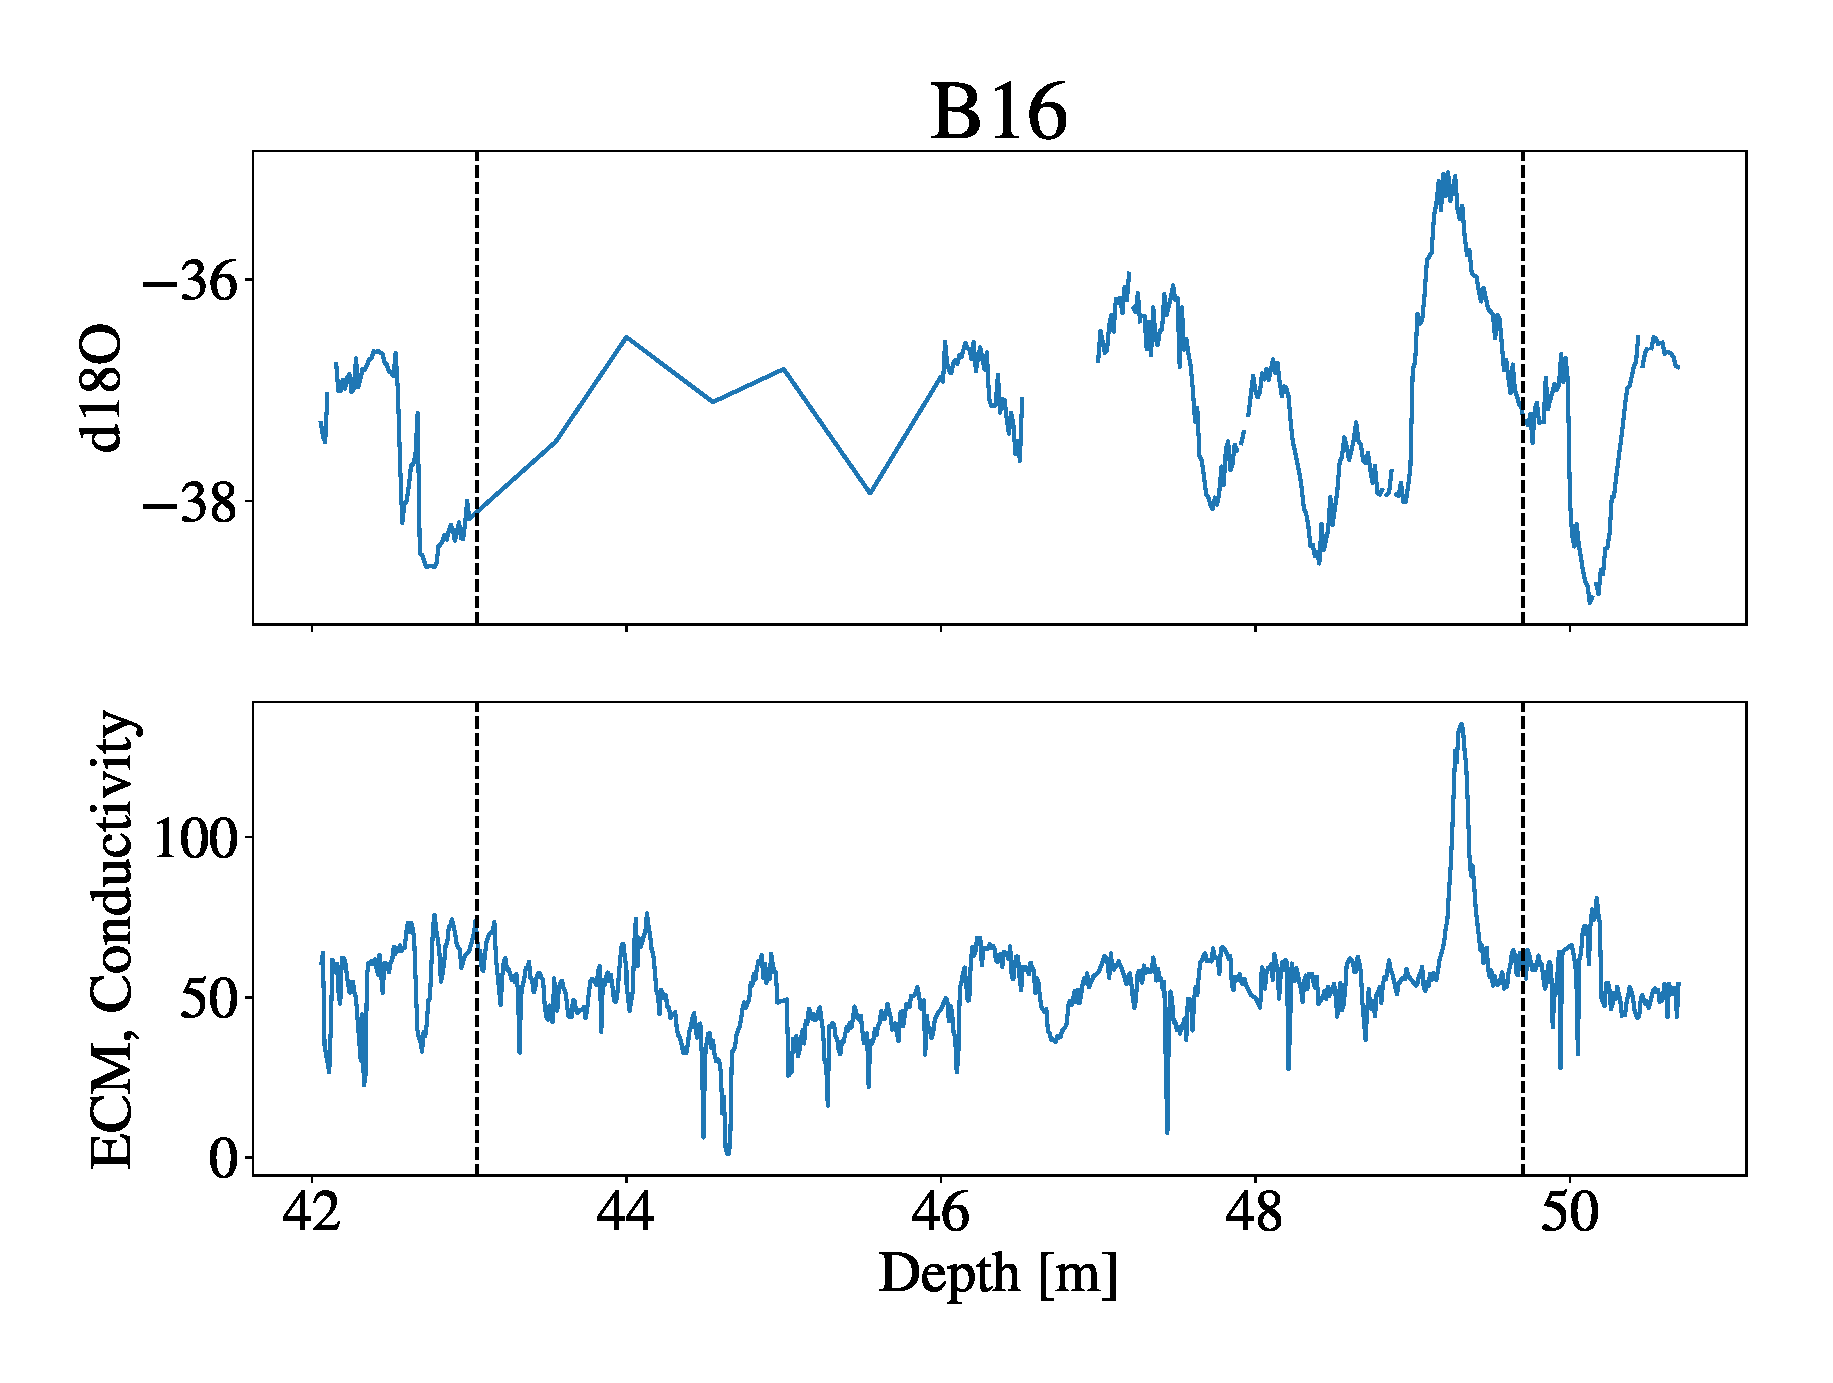
\includegraphics[width=0.7\textwidth]{Core_LT_B16.eps}
		\label{fig:B16}
	\caption{RESOLUTION: Maximum sample size (minimal resolution): 0.55 m = 55 cm. Minimum sample size(maximal resolution): 0.013 m = 1.3 cm. Unique sample sizes(7): $[0.013, 0.014, 0.015, 0.07,  0.1, 0.45, 0.55]$ m.\\
	LT LENGTH estimated: 6.65 m.\\
	Accumulation rate, range and mean.}
\end{figure}

\begin{figure}[h]
	\centering
	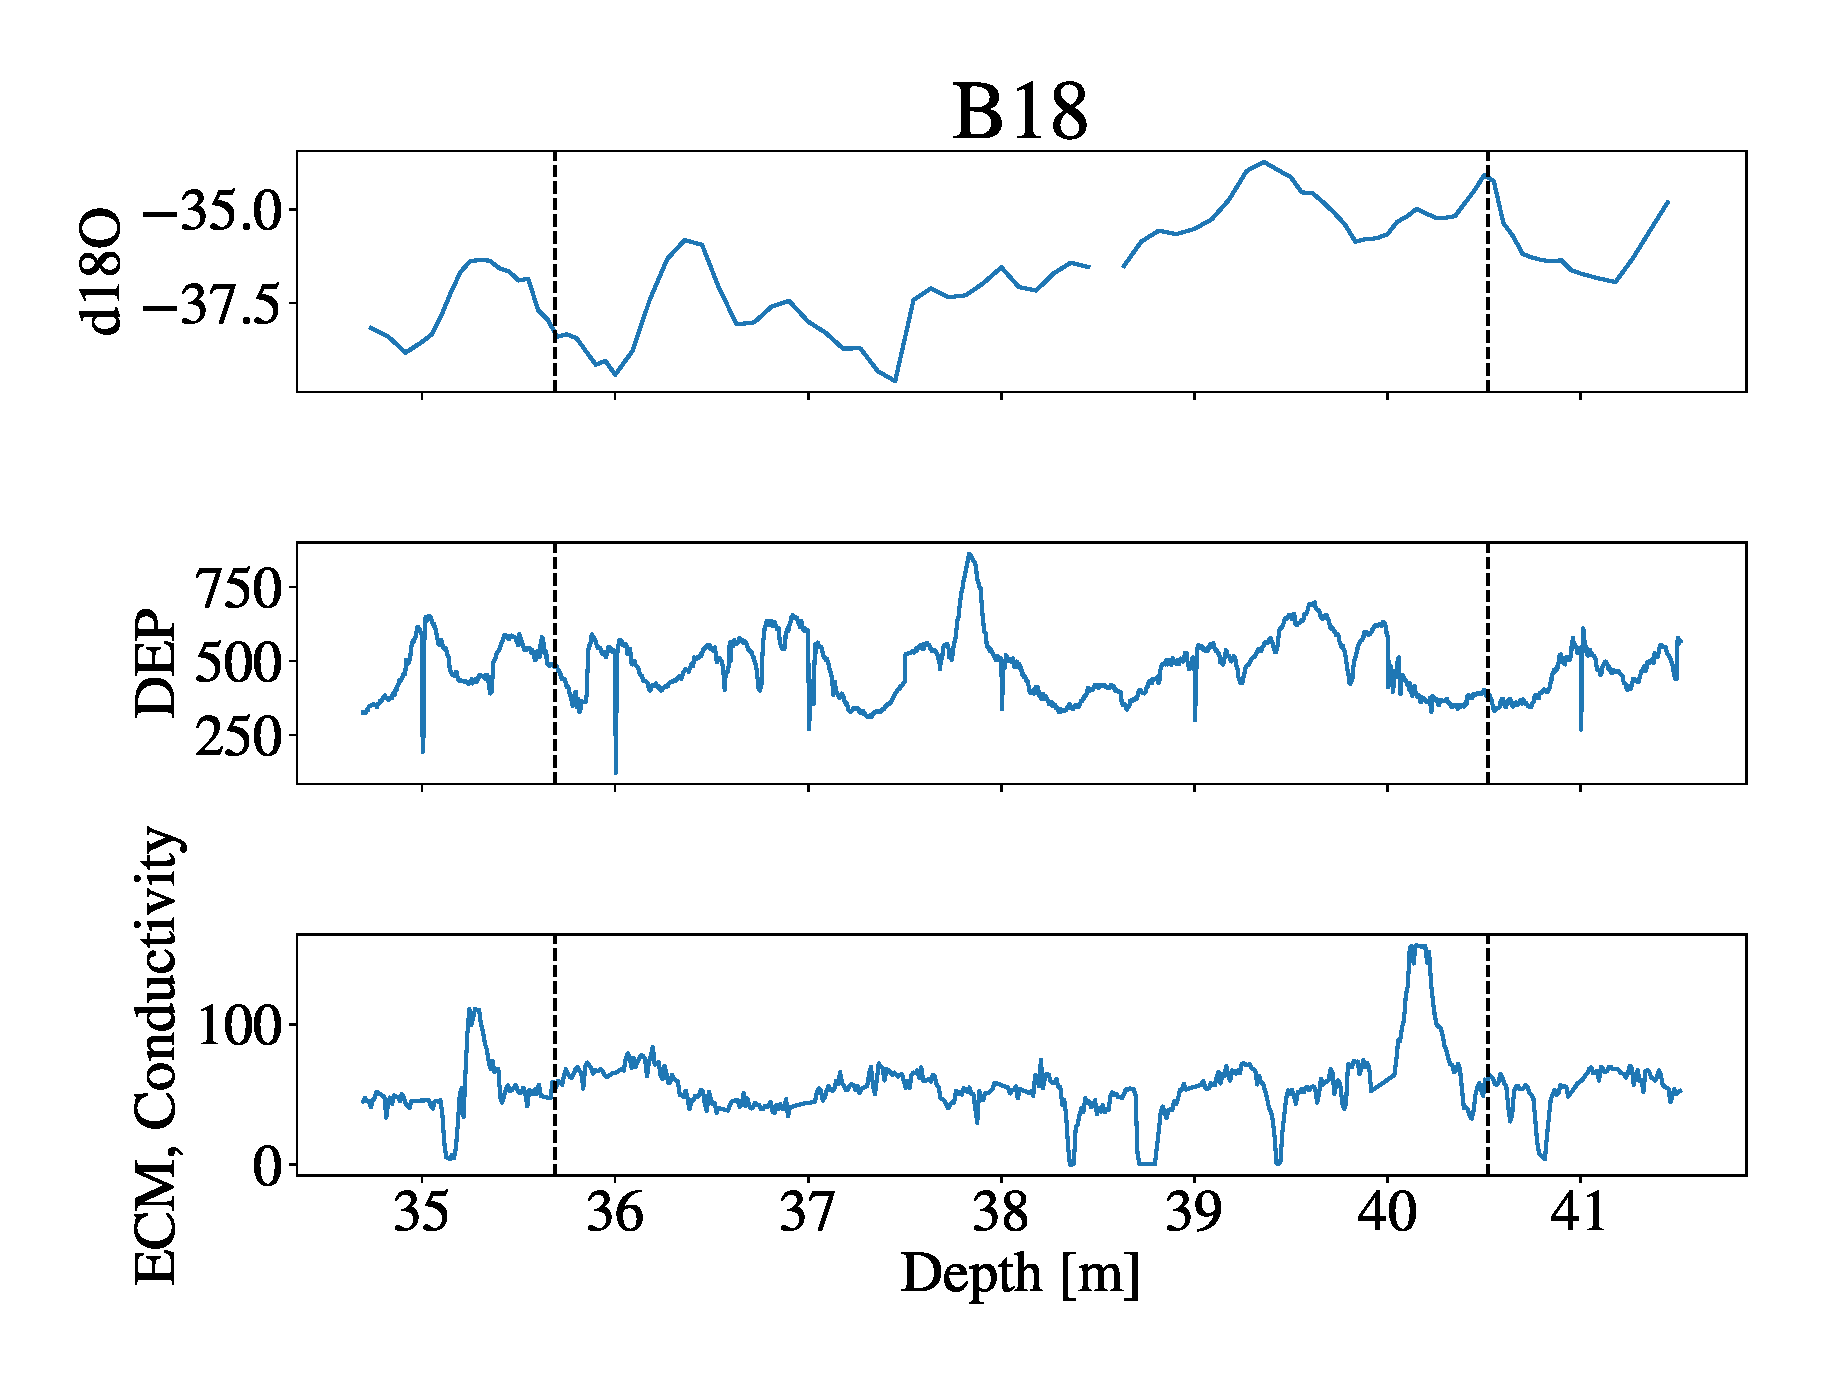
\includegraphics[width=0.7\textwidth]{Core_LT_B18.eps}
	\label{fig:B18}
	\caption{RESOLUTION: Maximum sample size (minimal resolution): 0.1 m = 10 cm. Minimum sample size(maximal resolution): 0.05 m = 5 cm. Unique sample sizes(6): $[0.05, 0.0555, 0.0556, 0.09, 0.095, 0.1]$ m.\\
	LT LENGTH estimated: 4.83 m.\\
	Accumulation rate, range and mean.}
\end{figure}

\begin{figure}[h]
	\centering
	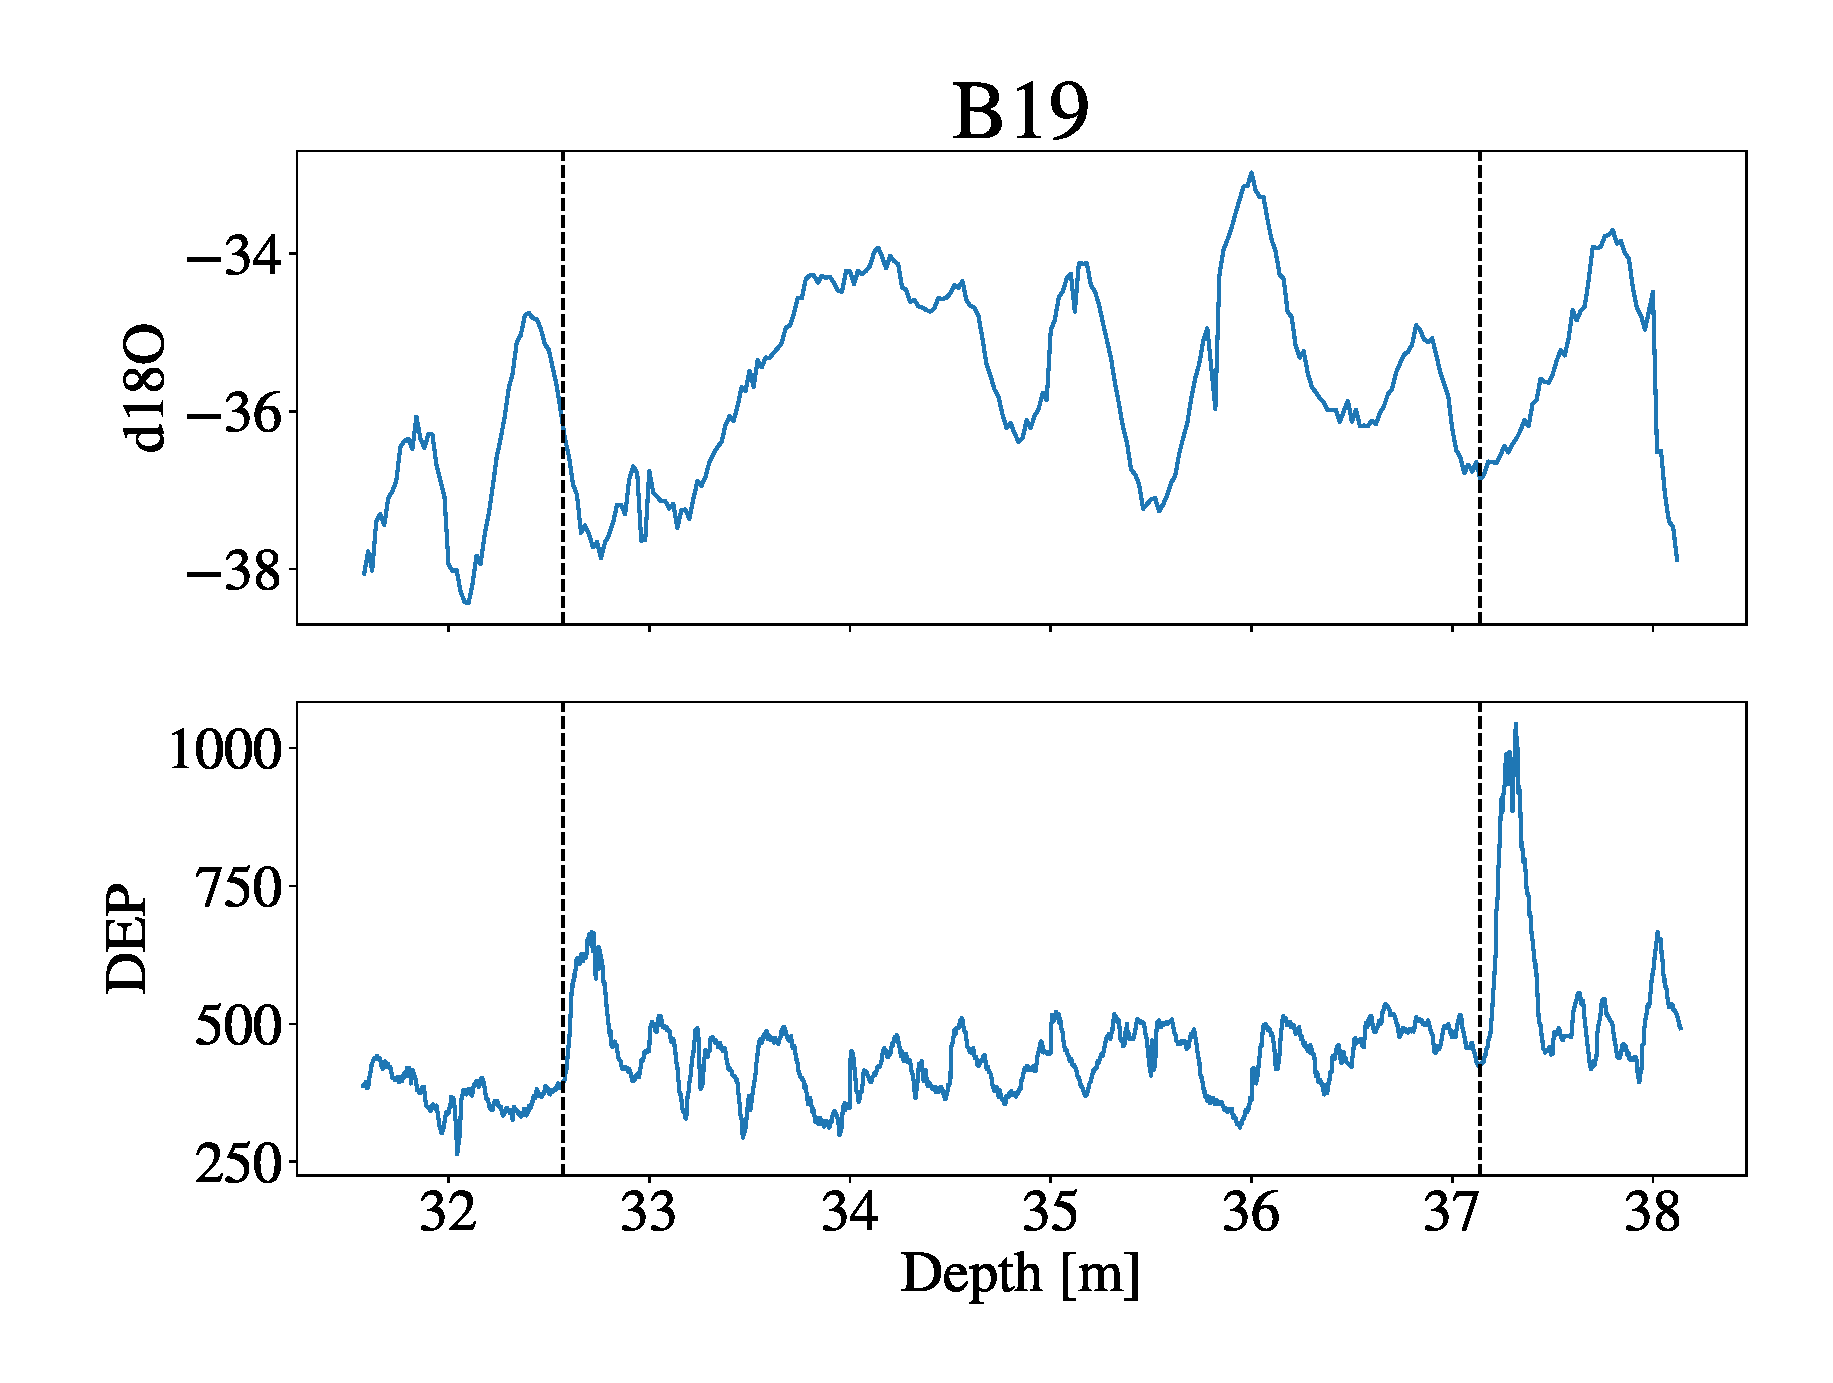
\includegraphics[width=0.7\textwidth]{Core_LT_B19.eps}
		\label{fig:B19}
	\caption{RESOLUTION: Maximum sample size (minimal resolution): 0.02 m = 2 cm. Minimum sample size(maximal resolution): 0.02 m = 2 cm. Unique sample sizes(1): $[0.02]$ m.\\
	LT LENGTH estimated: 4.57 m.\\
	Accumulation rate, range and mean.}
\end{figure}

\begin{figure}[h]
	\centering
	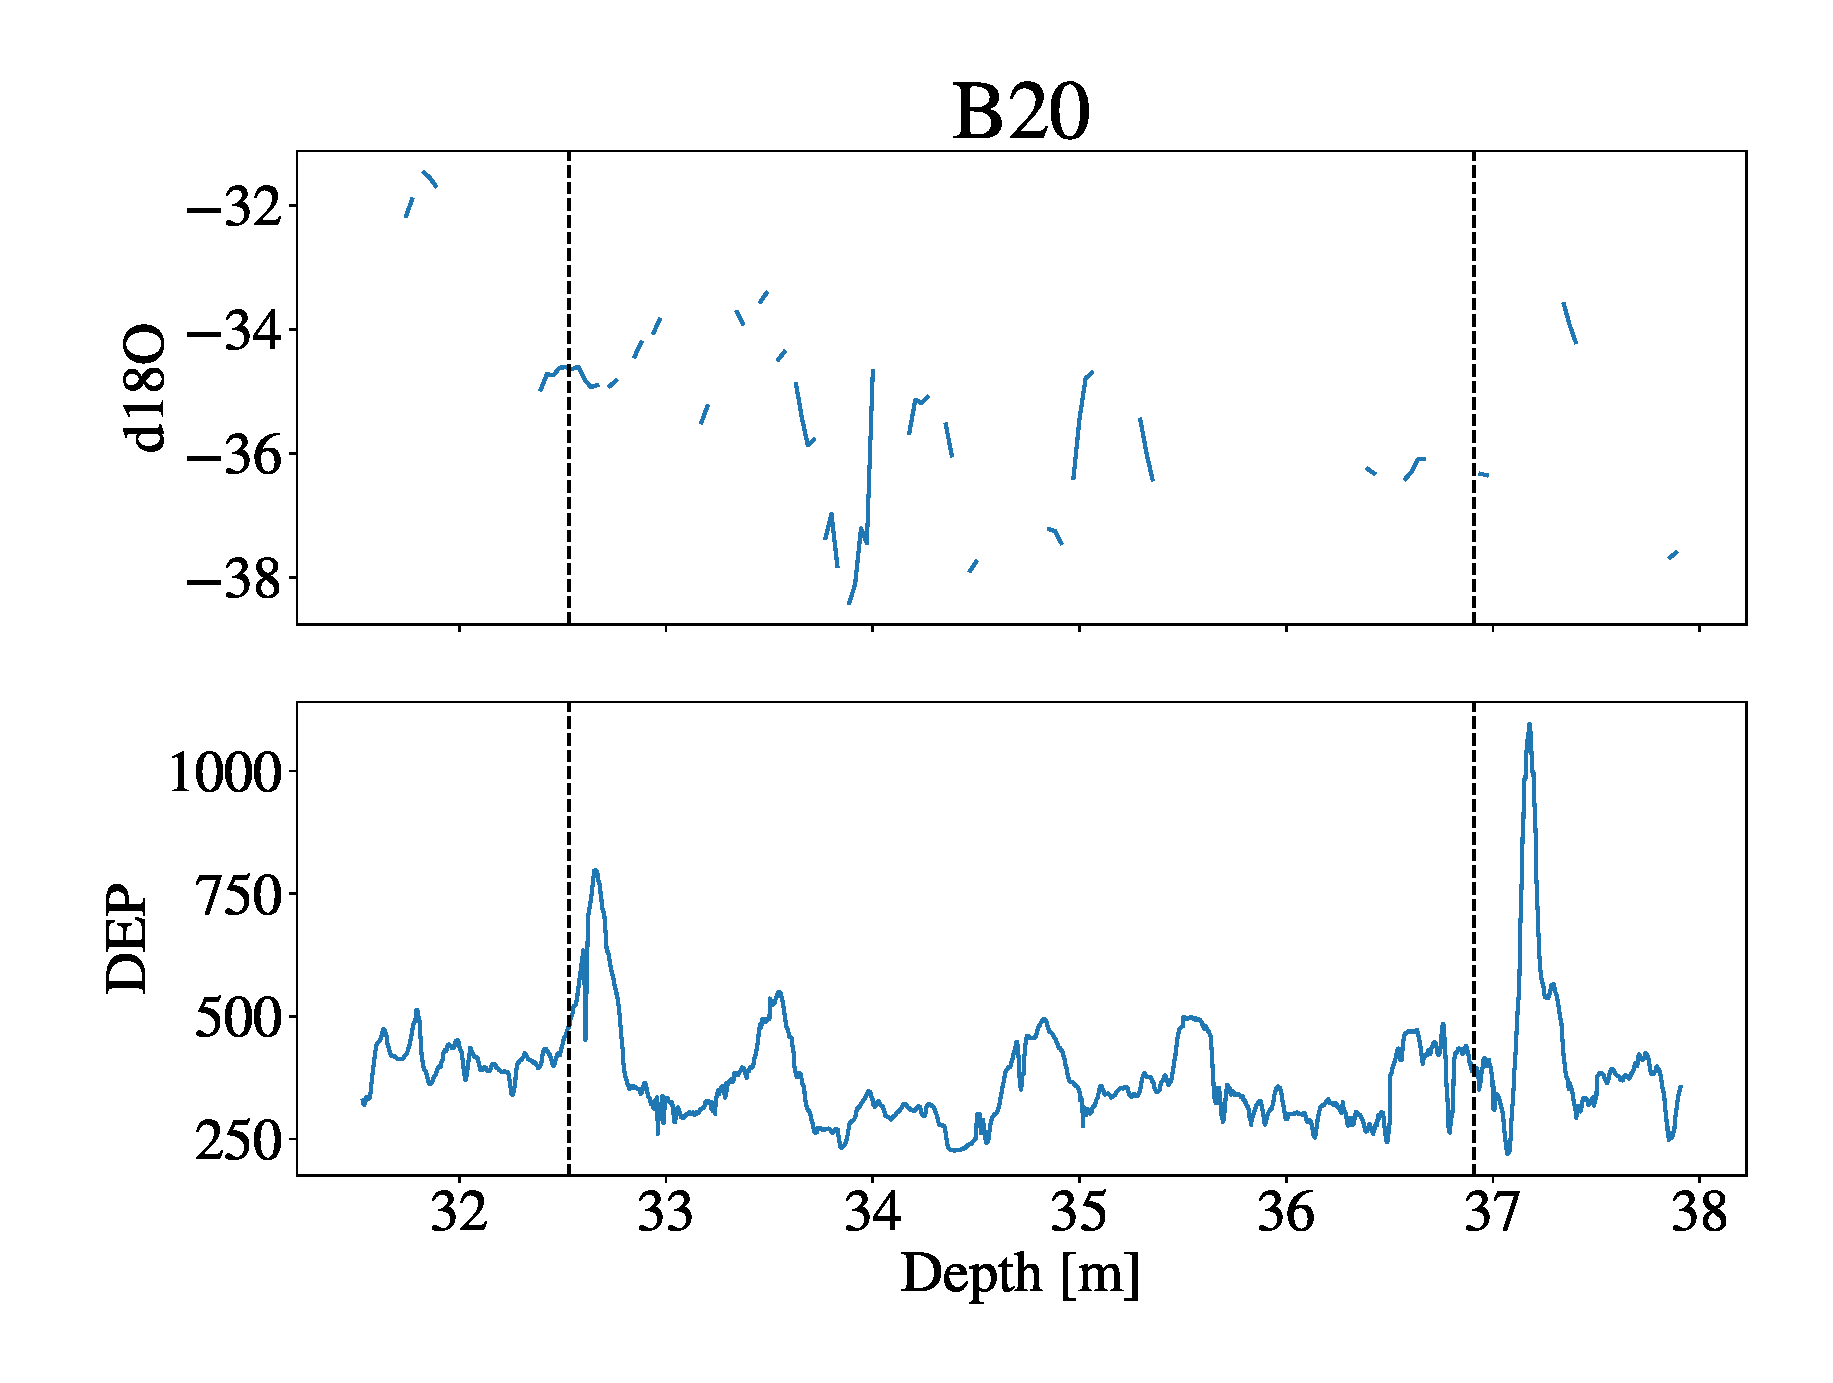
\includegraphics[width=0.7\textwidth]{Core_LT_B20.eps}
	\label{fig:B20}
	\caption{RESOLUTION: Maximum sample size (minimal resolution): 0.0304 m = 3.04 cm. Minimum sample size(maximal resolution): 0.0285 m = 2.85 cm. Unique sample sizes(6): $[0.0285, 0.0286, 0.0294, 0.0295, 0.0303, 0.0304]$ m.\\
	LT LENGTH estimated: 4.38 m.\\
	Accumulation rate, range and mean.}
	
\end{figure}

\begin{figure}[h]
	\centering
	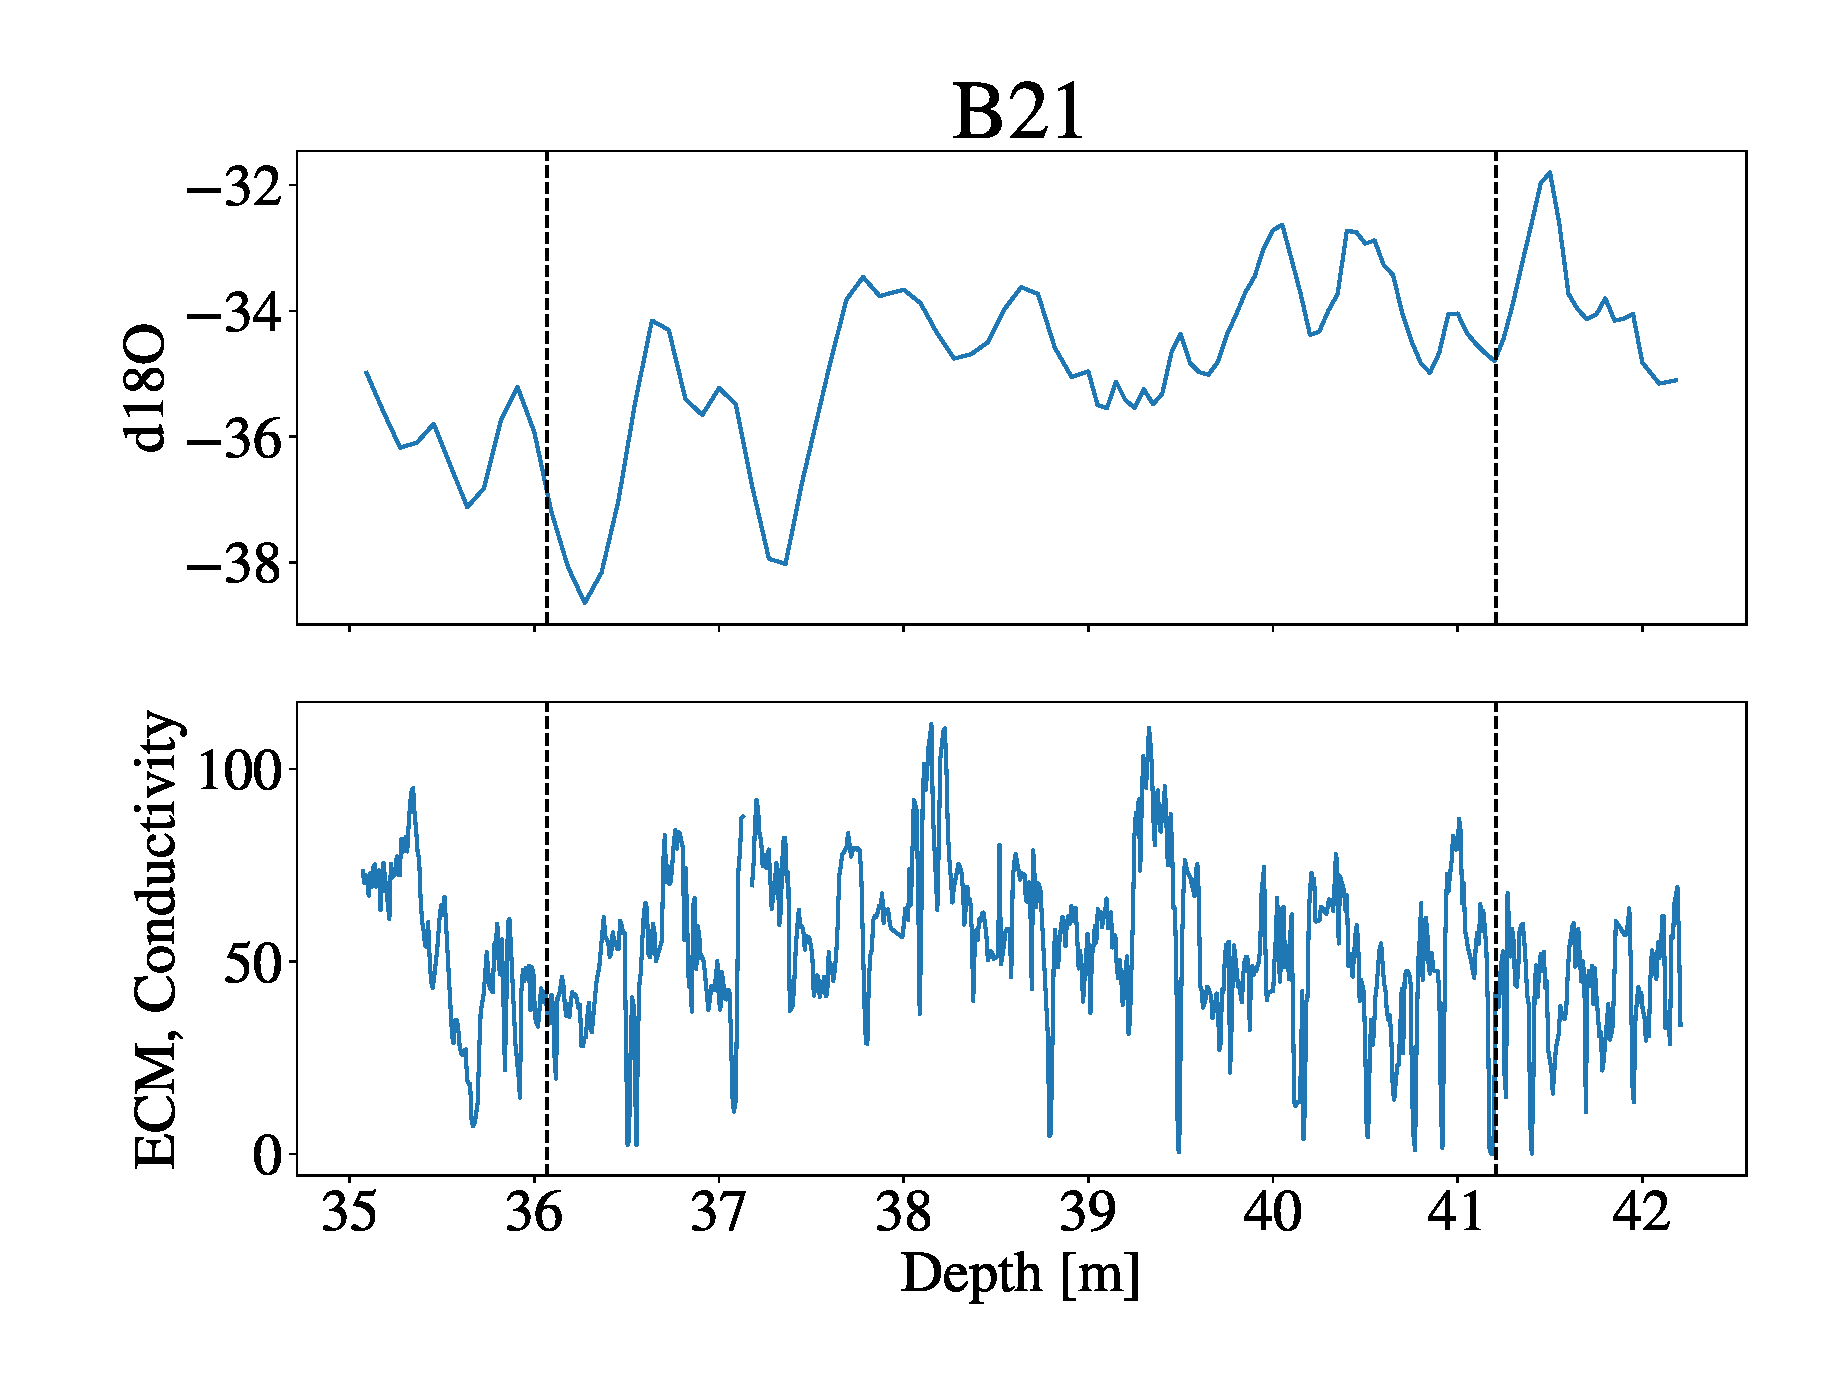
\includegraphics[width=0.7\textwidth]{Core_LT_B21.eps}
	\label{fig:B21}
	\caption{RESOLUTION: Maximum sample size (minimal resolution): 0.15 m = 15 cm. Minimum sample size(maximal resolution): 0.05 m = 5 cm. Unique sample sizes(5): $[0.05, 0.09, 0.0909, 0.13, 0.15]$ m.\\
		LT LENGTH estimated: 5.14 m.\\
		Accumulation rate, range and mean.}
\end{figure}

\begin{figure}[h]
	\centering
	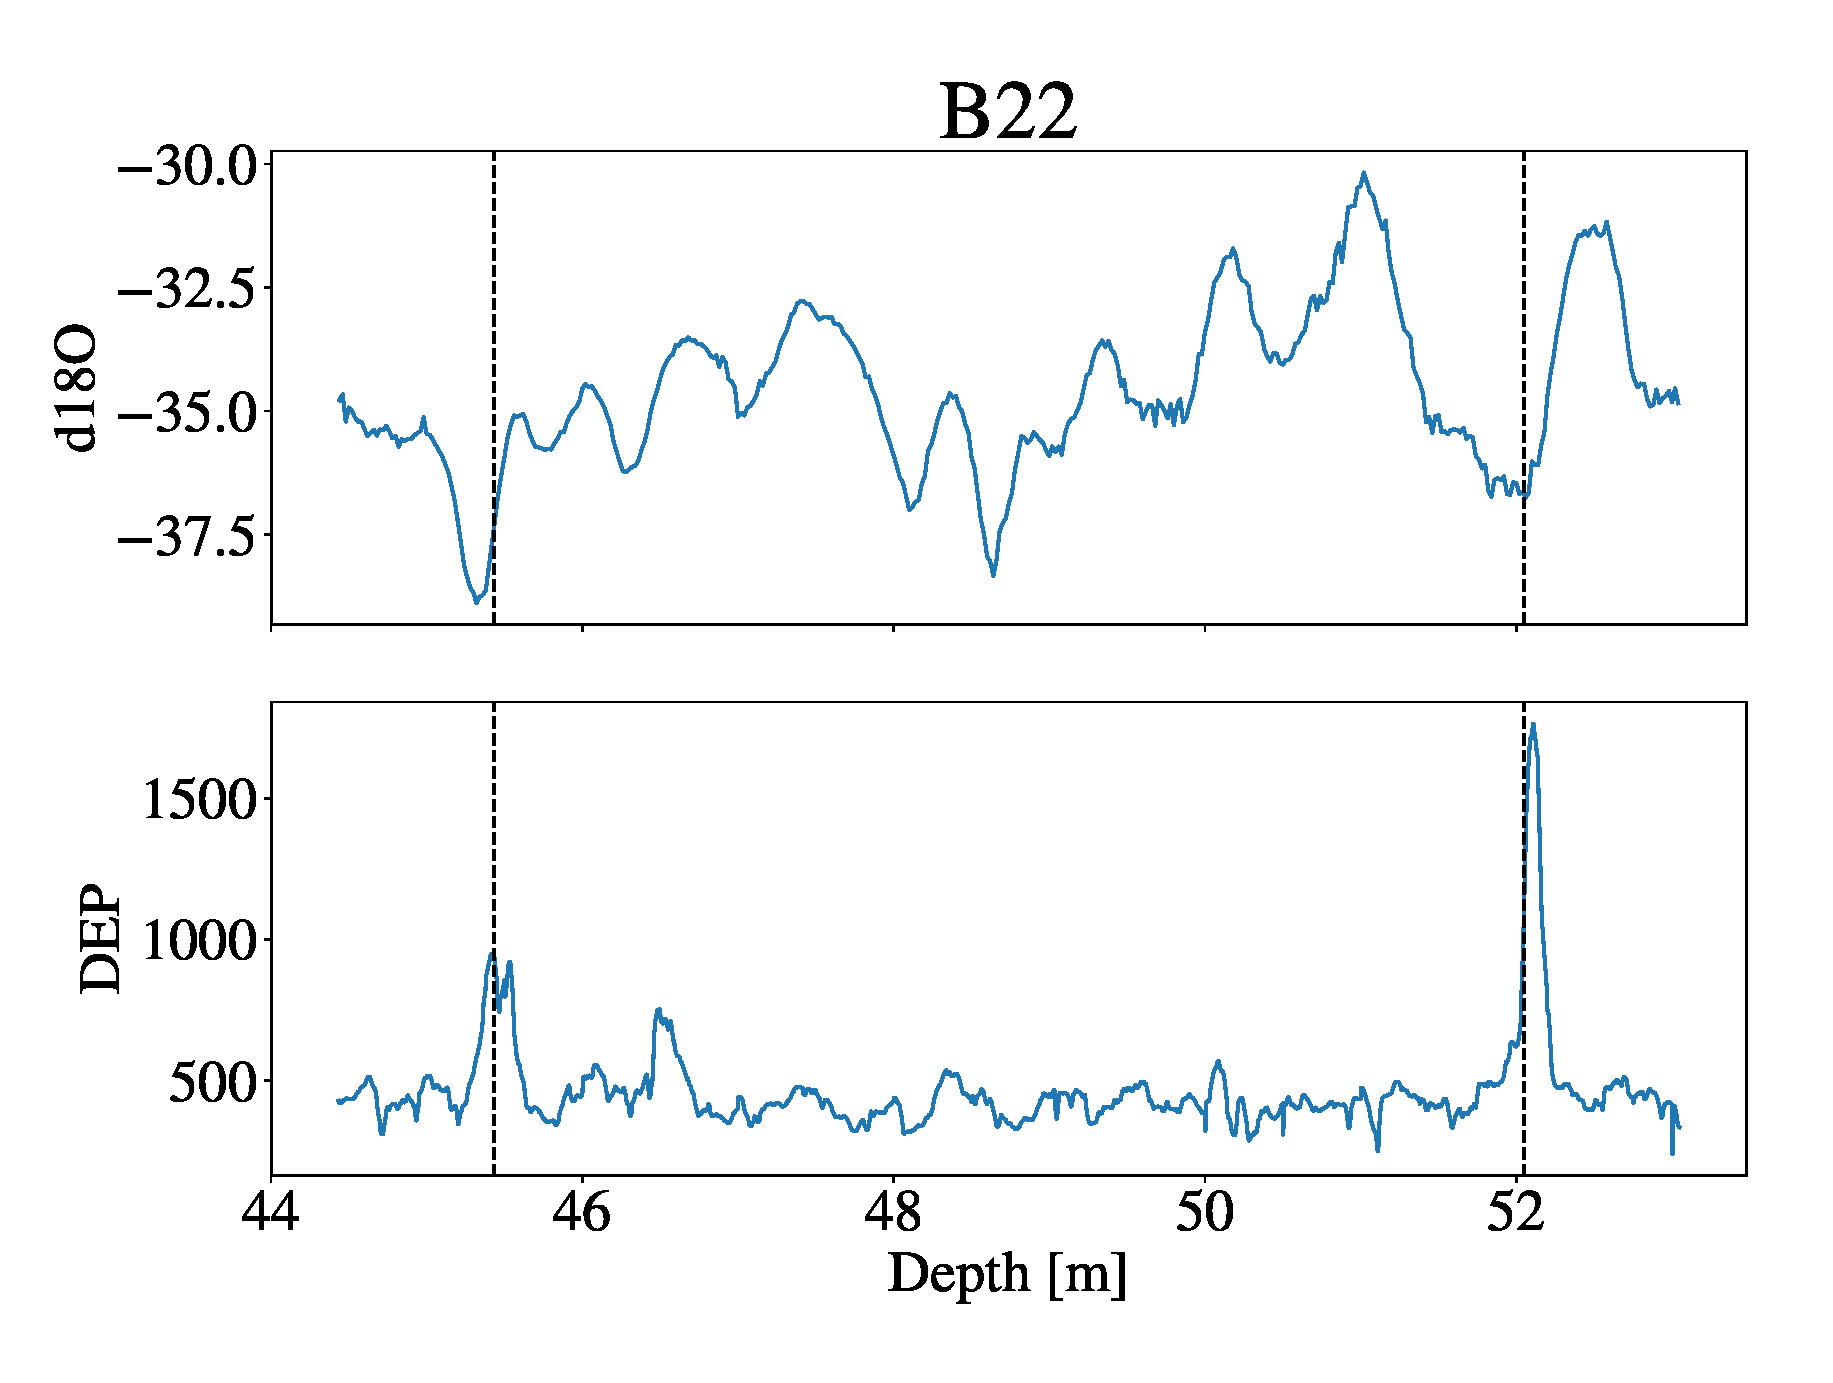
\includegraphics[width=0.7\textwidth]{Core_LT_B22.eps}
	\label{fig:B22}
	\caption{RESOLUTION: Maximum sample size (minimal resolution): 0.02 m = 2 cm. Minimum sample size(maximal resolution): 0.02 m = 2 cm. Unique sample sizes(1): $[0.02]$ m.\\
		LT LENGTH estimated: 6.62 m.\\
		Accumulation rate, range and mean.}	
\end{figure}

\begin{figure}[h]
	\centering
	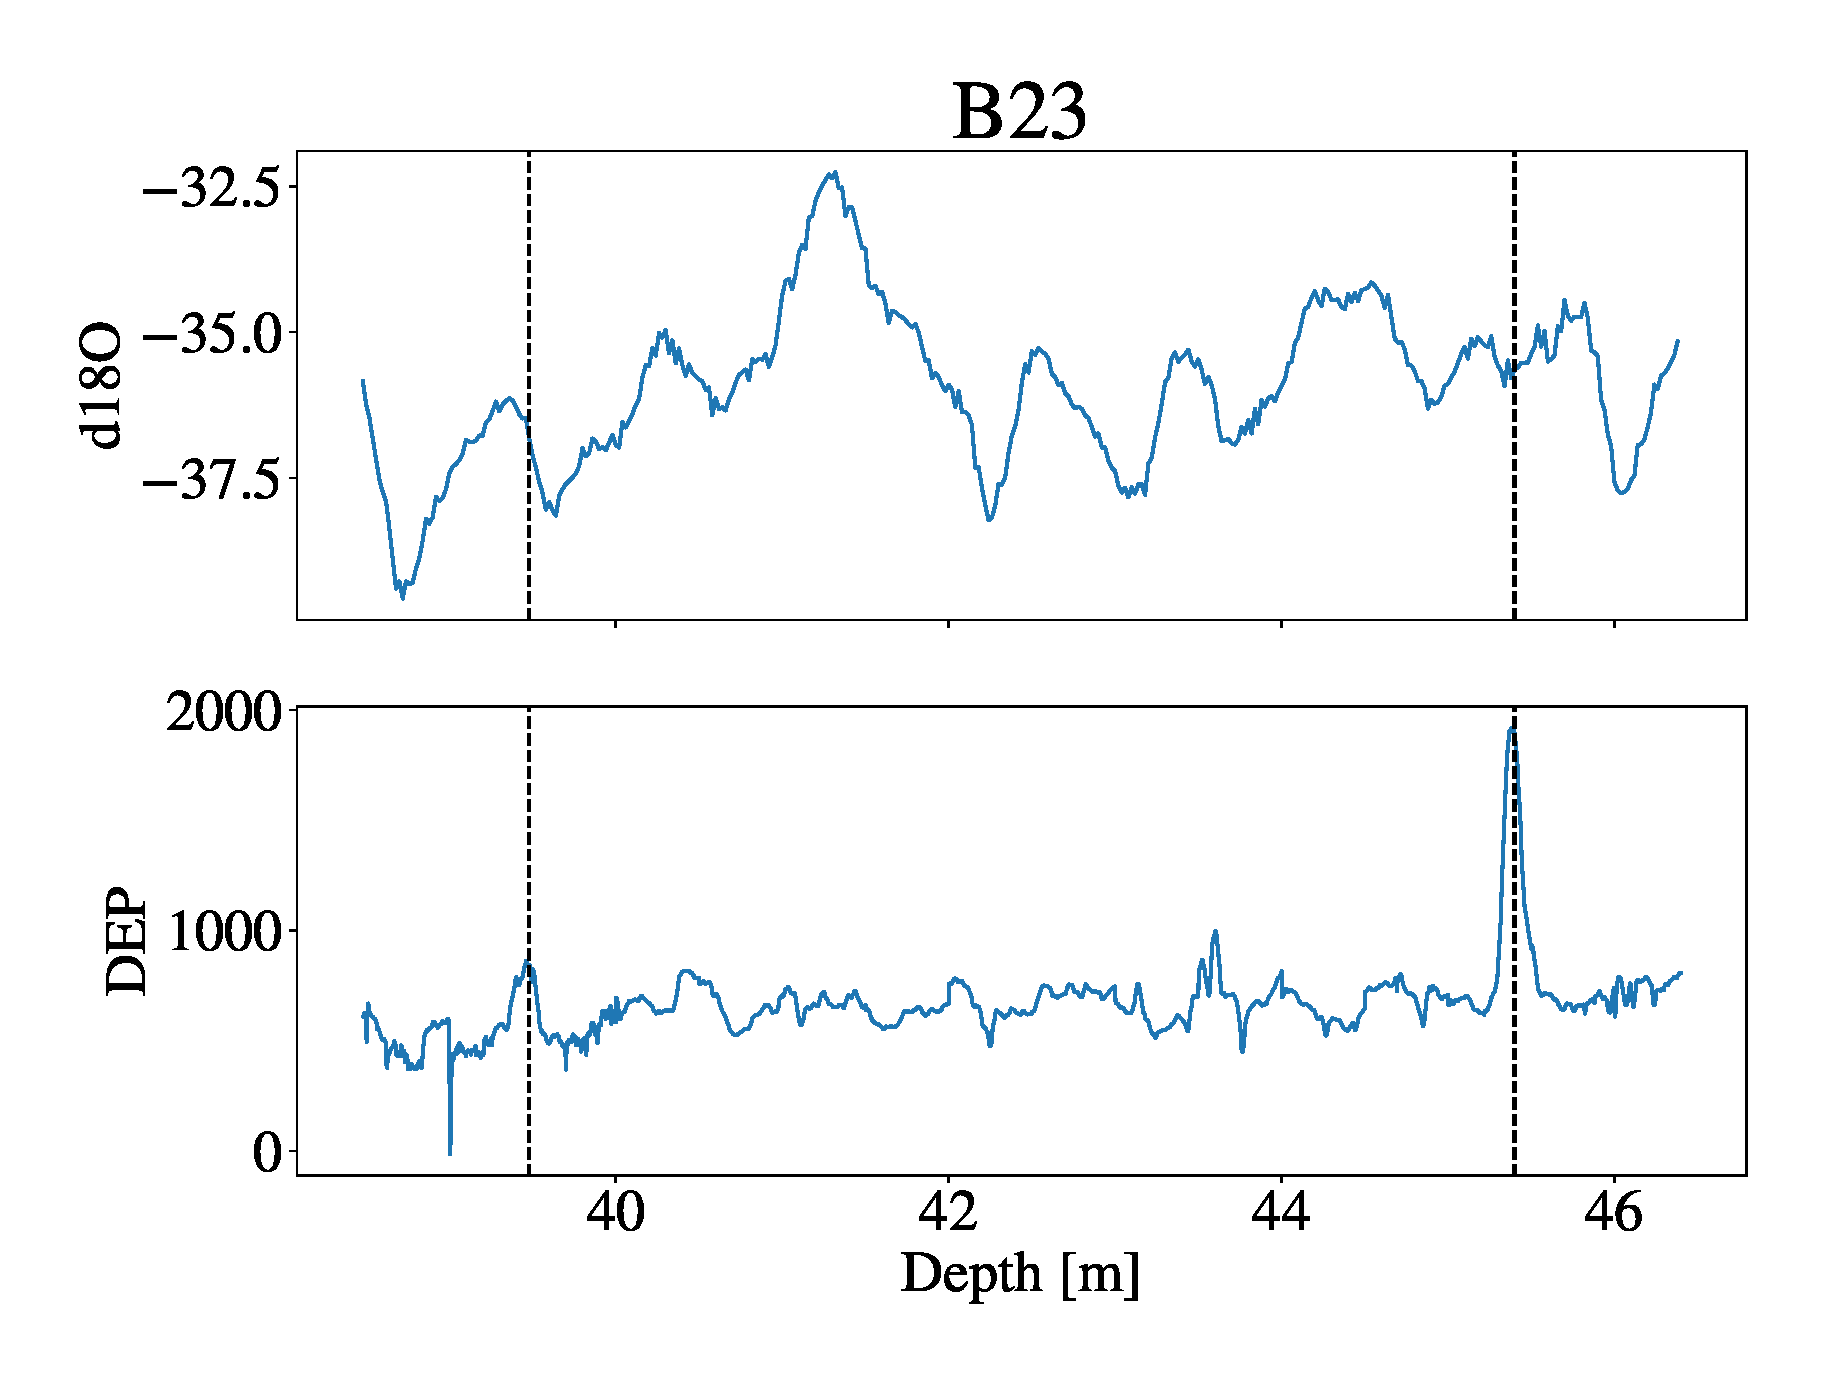
\includegraphics[width=0.7\textwidth]{Core_LT_B23.eps}
	\label{fig:B23}
	\caption{RESOLUTION: Maximum sample size (minimal resolution): 0.02 m = 2 cm. Minimum sample size(maximal resolution): 0.02 m = 2 cm. Unique sample sizes(1): $[0.02]$ m.\\
		LT LENGTH estimated: 5.92 m.\\
		Accumulation rate, range and mean.}
\end{figure}
\newpage
\begin{rotatepage}
	\begin{landscape}
		\begin{table}
			\centering
			\begin{tabular}{c||c||c}
				\textcolor{BrickRed}{\textbf{TERRIBLE}} & \textcolor{YellowOrange}{\textbf{REASONABLE}} & \textcolor{OliveGreen}{\textbf{GOOD}} \\
				\hline
				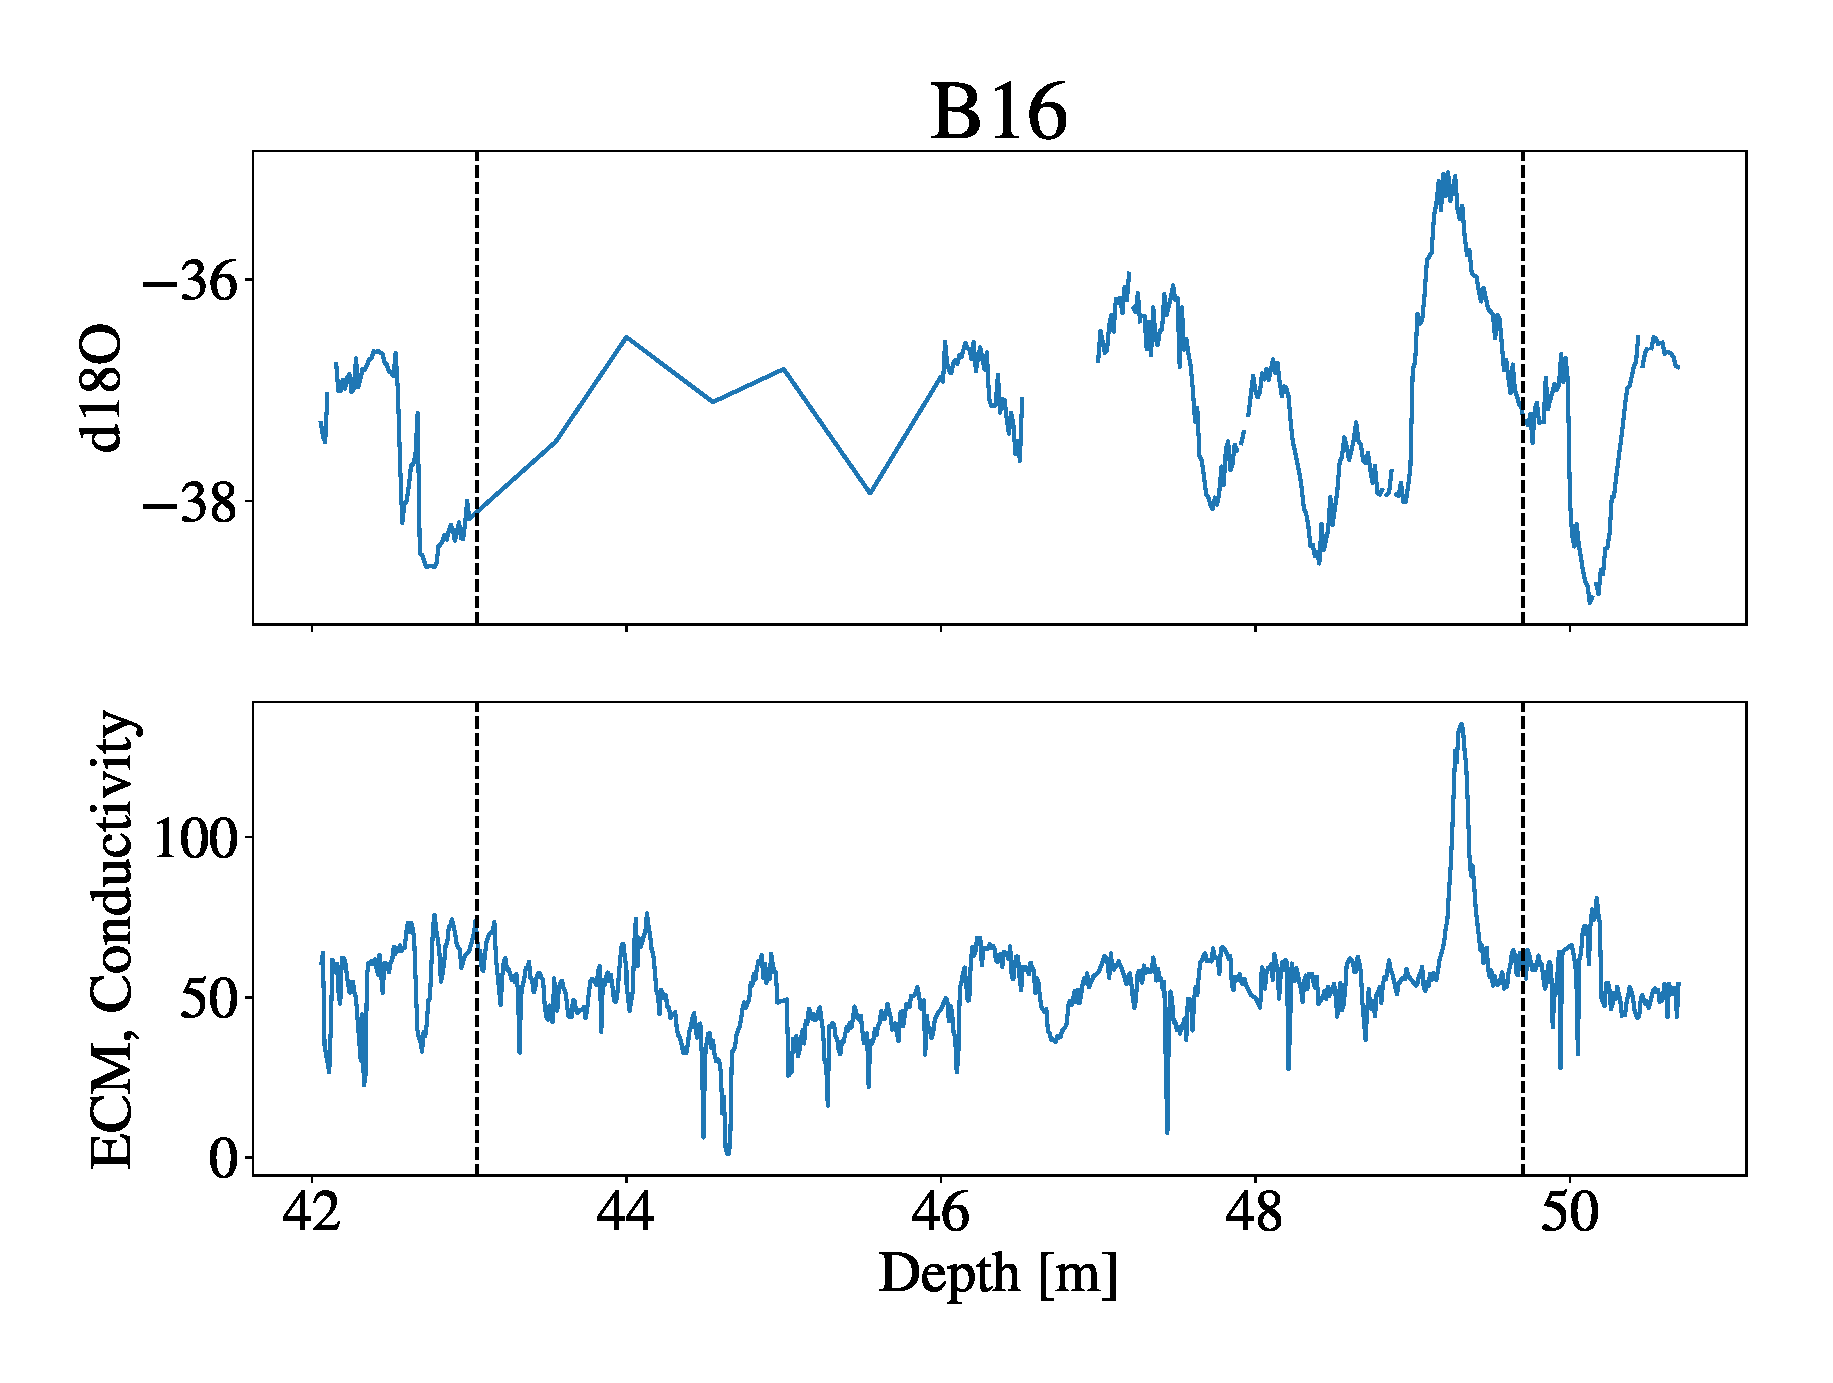
\includegraphics[width =0.3\linewidth]{Core_LT_B16.eps} & 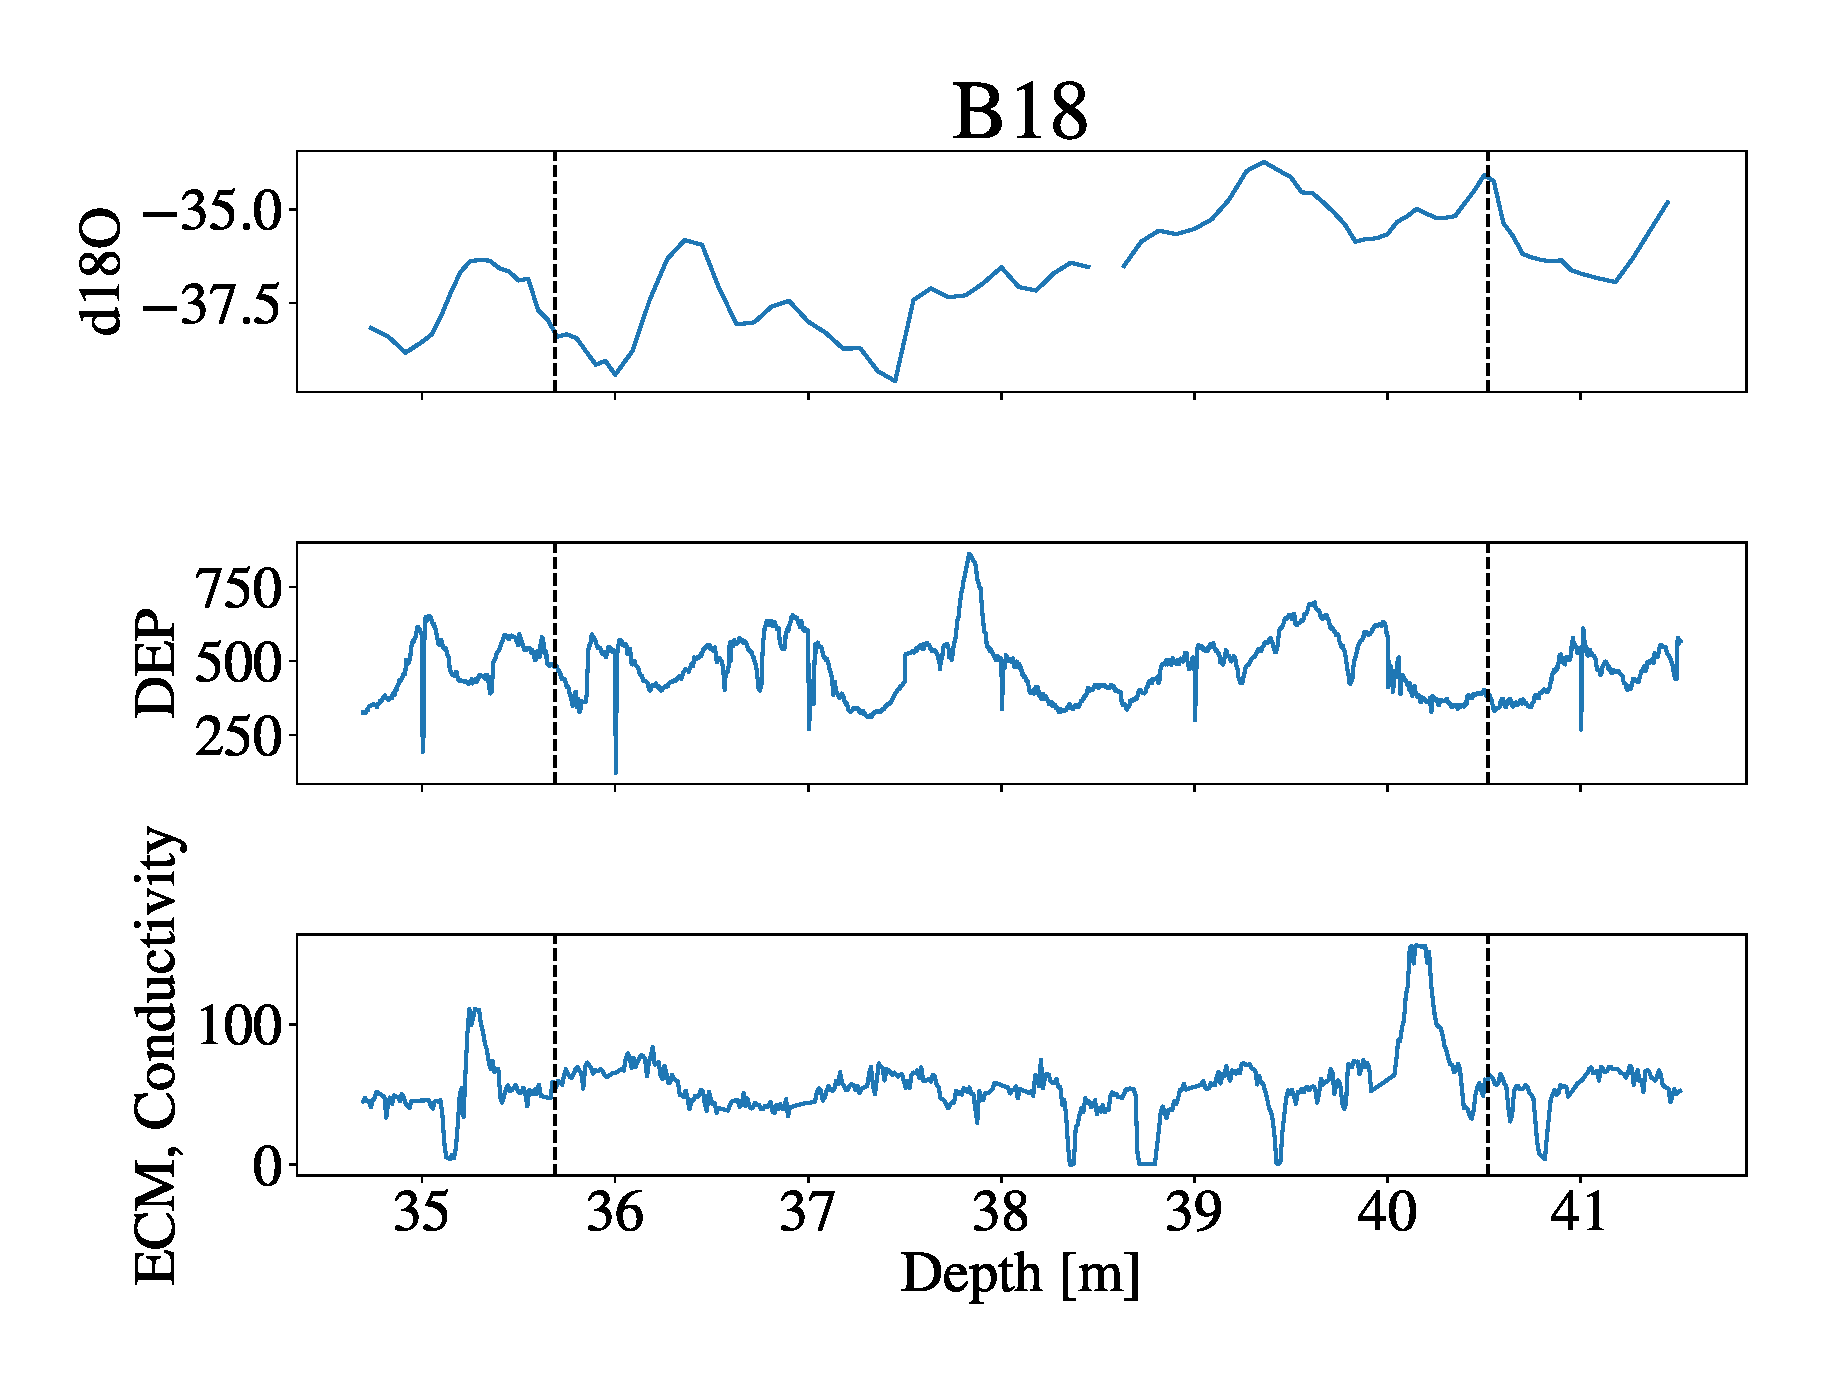
\includegraphics[width =0.3\linewidth]{Core_LT_B18.eps} & 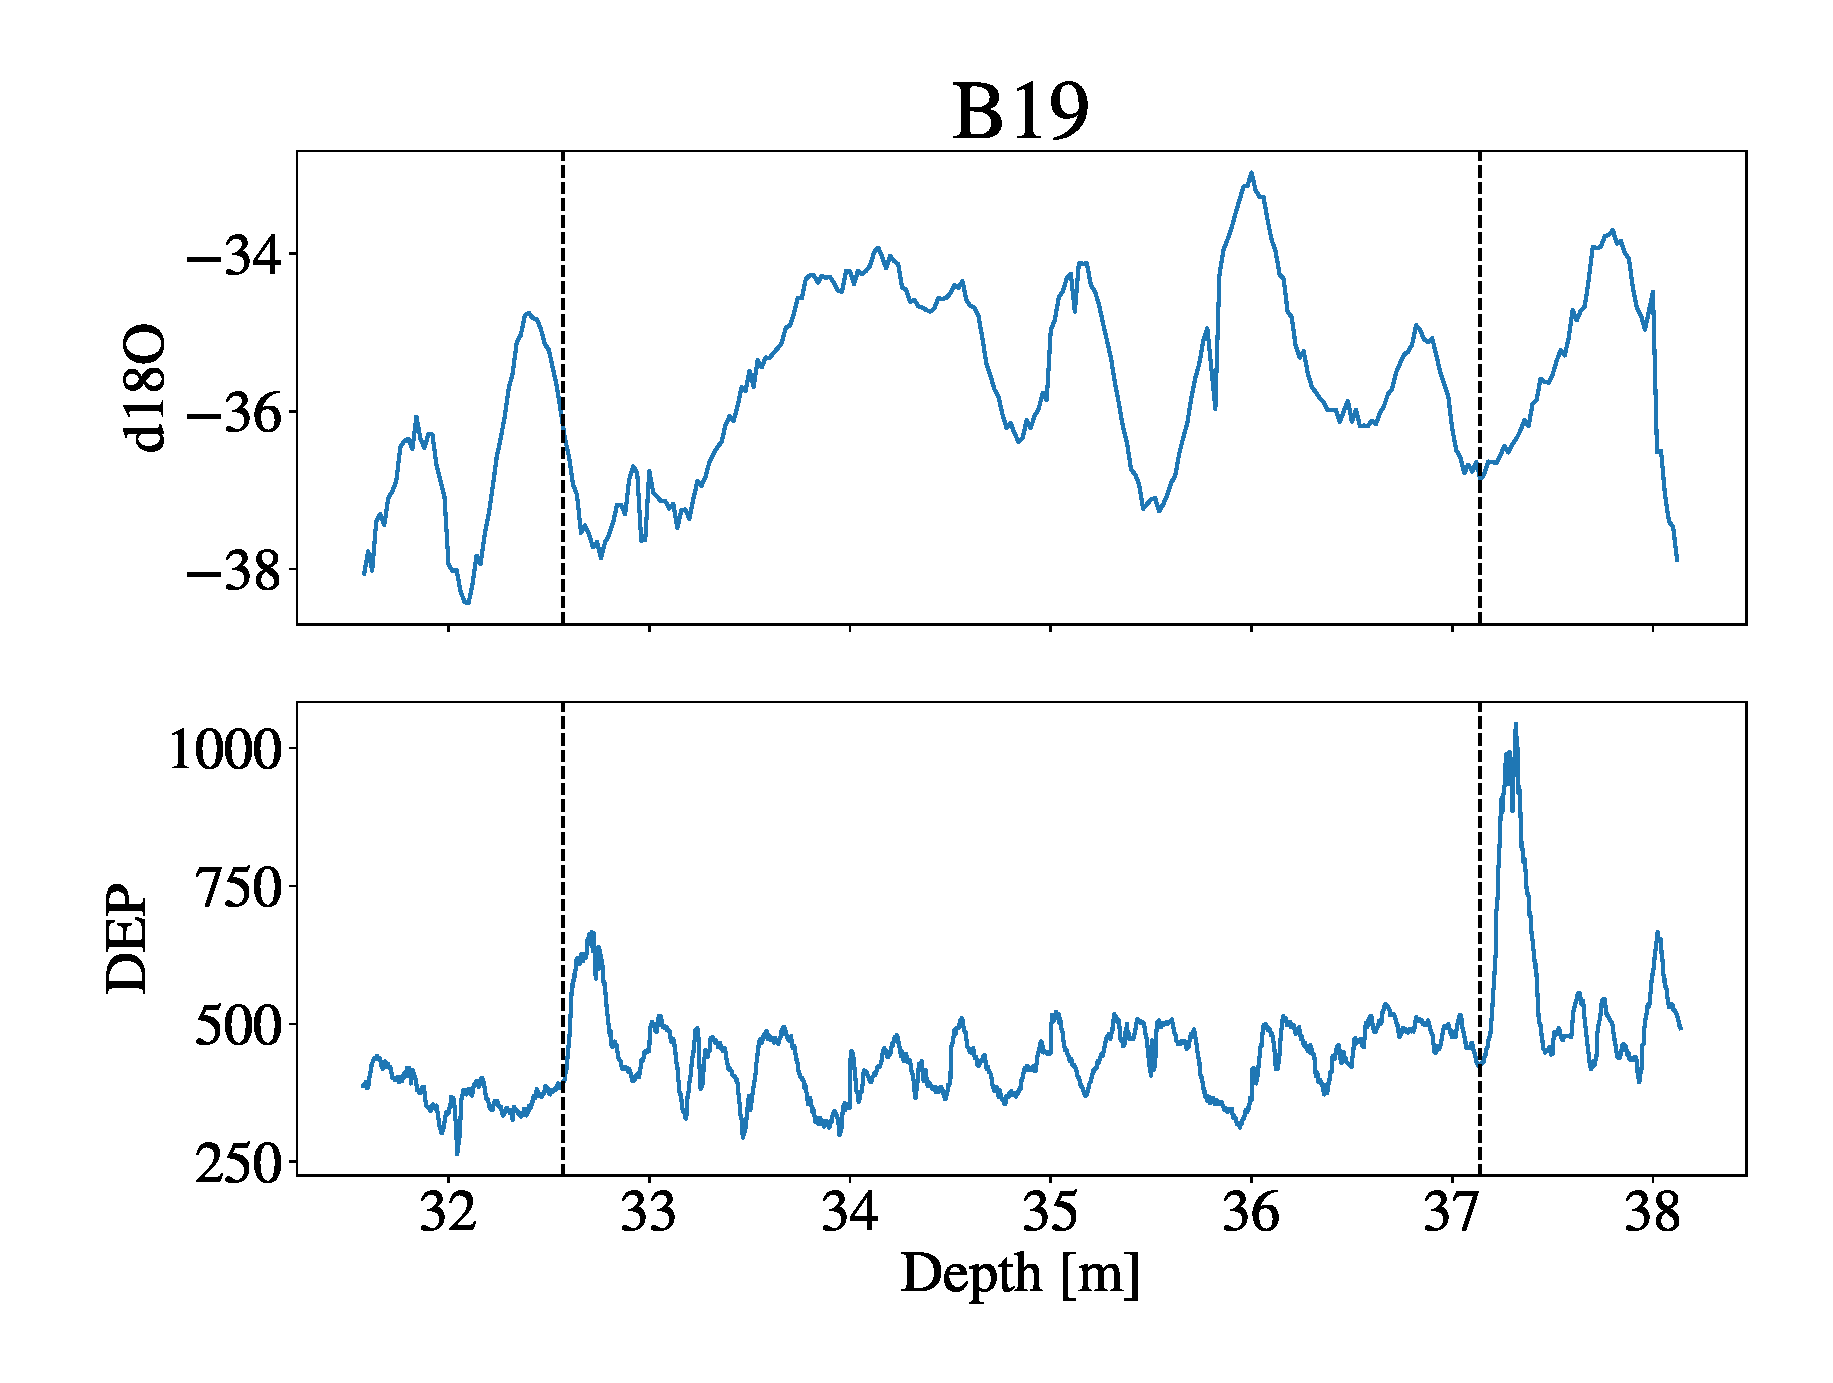
\includegraphics[width =0.3\linewidth]{Core_LT_B19.eps} \\
				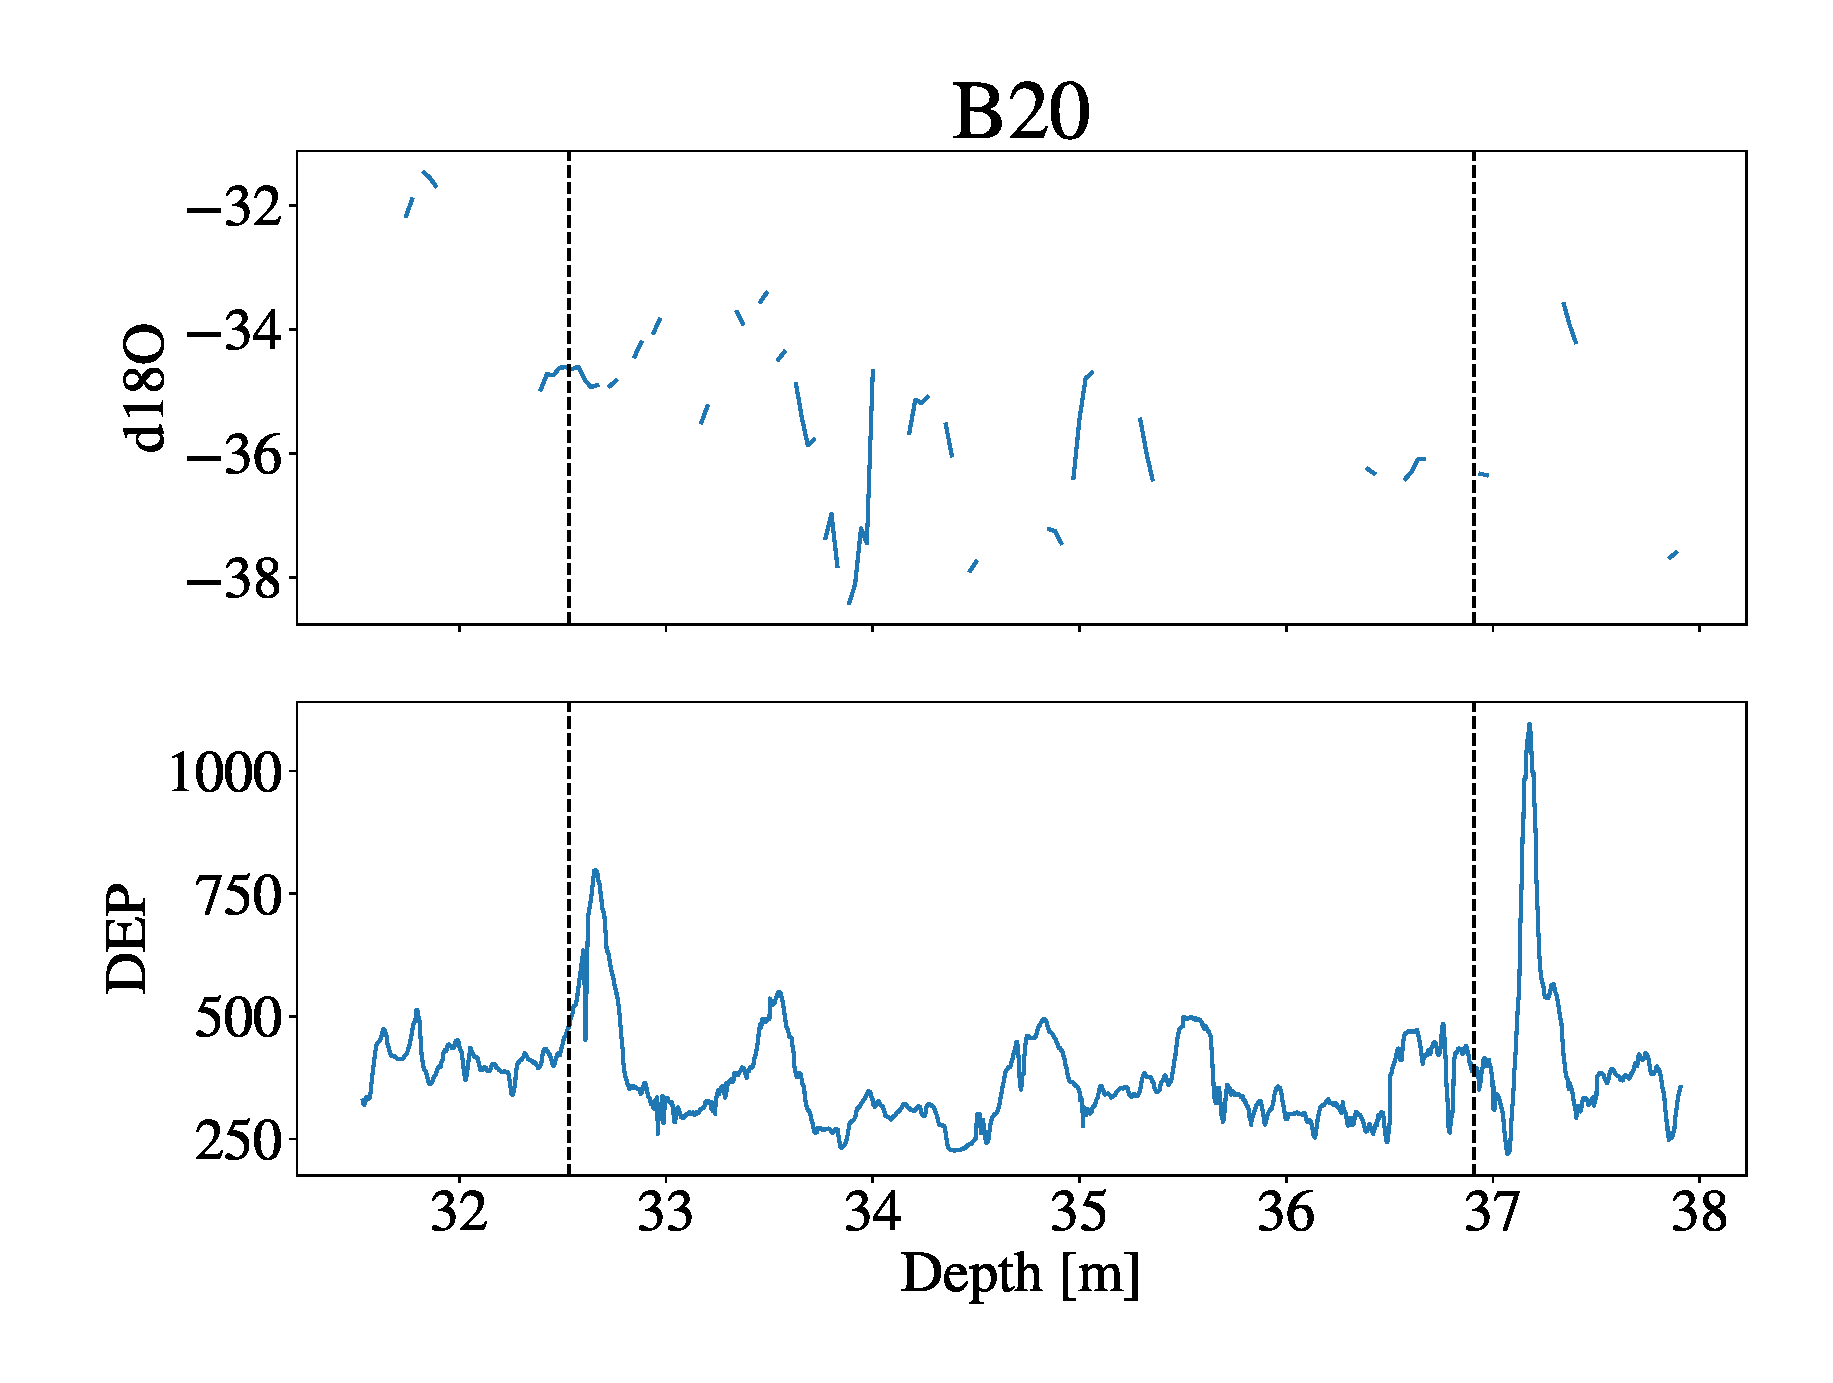
\includegraphics[width =0.3\linewidth]{Core_LT_B20.eps} & 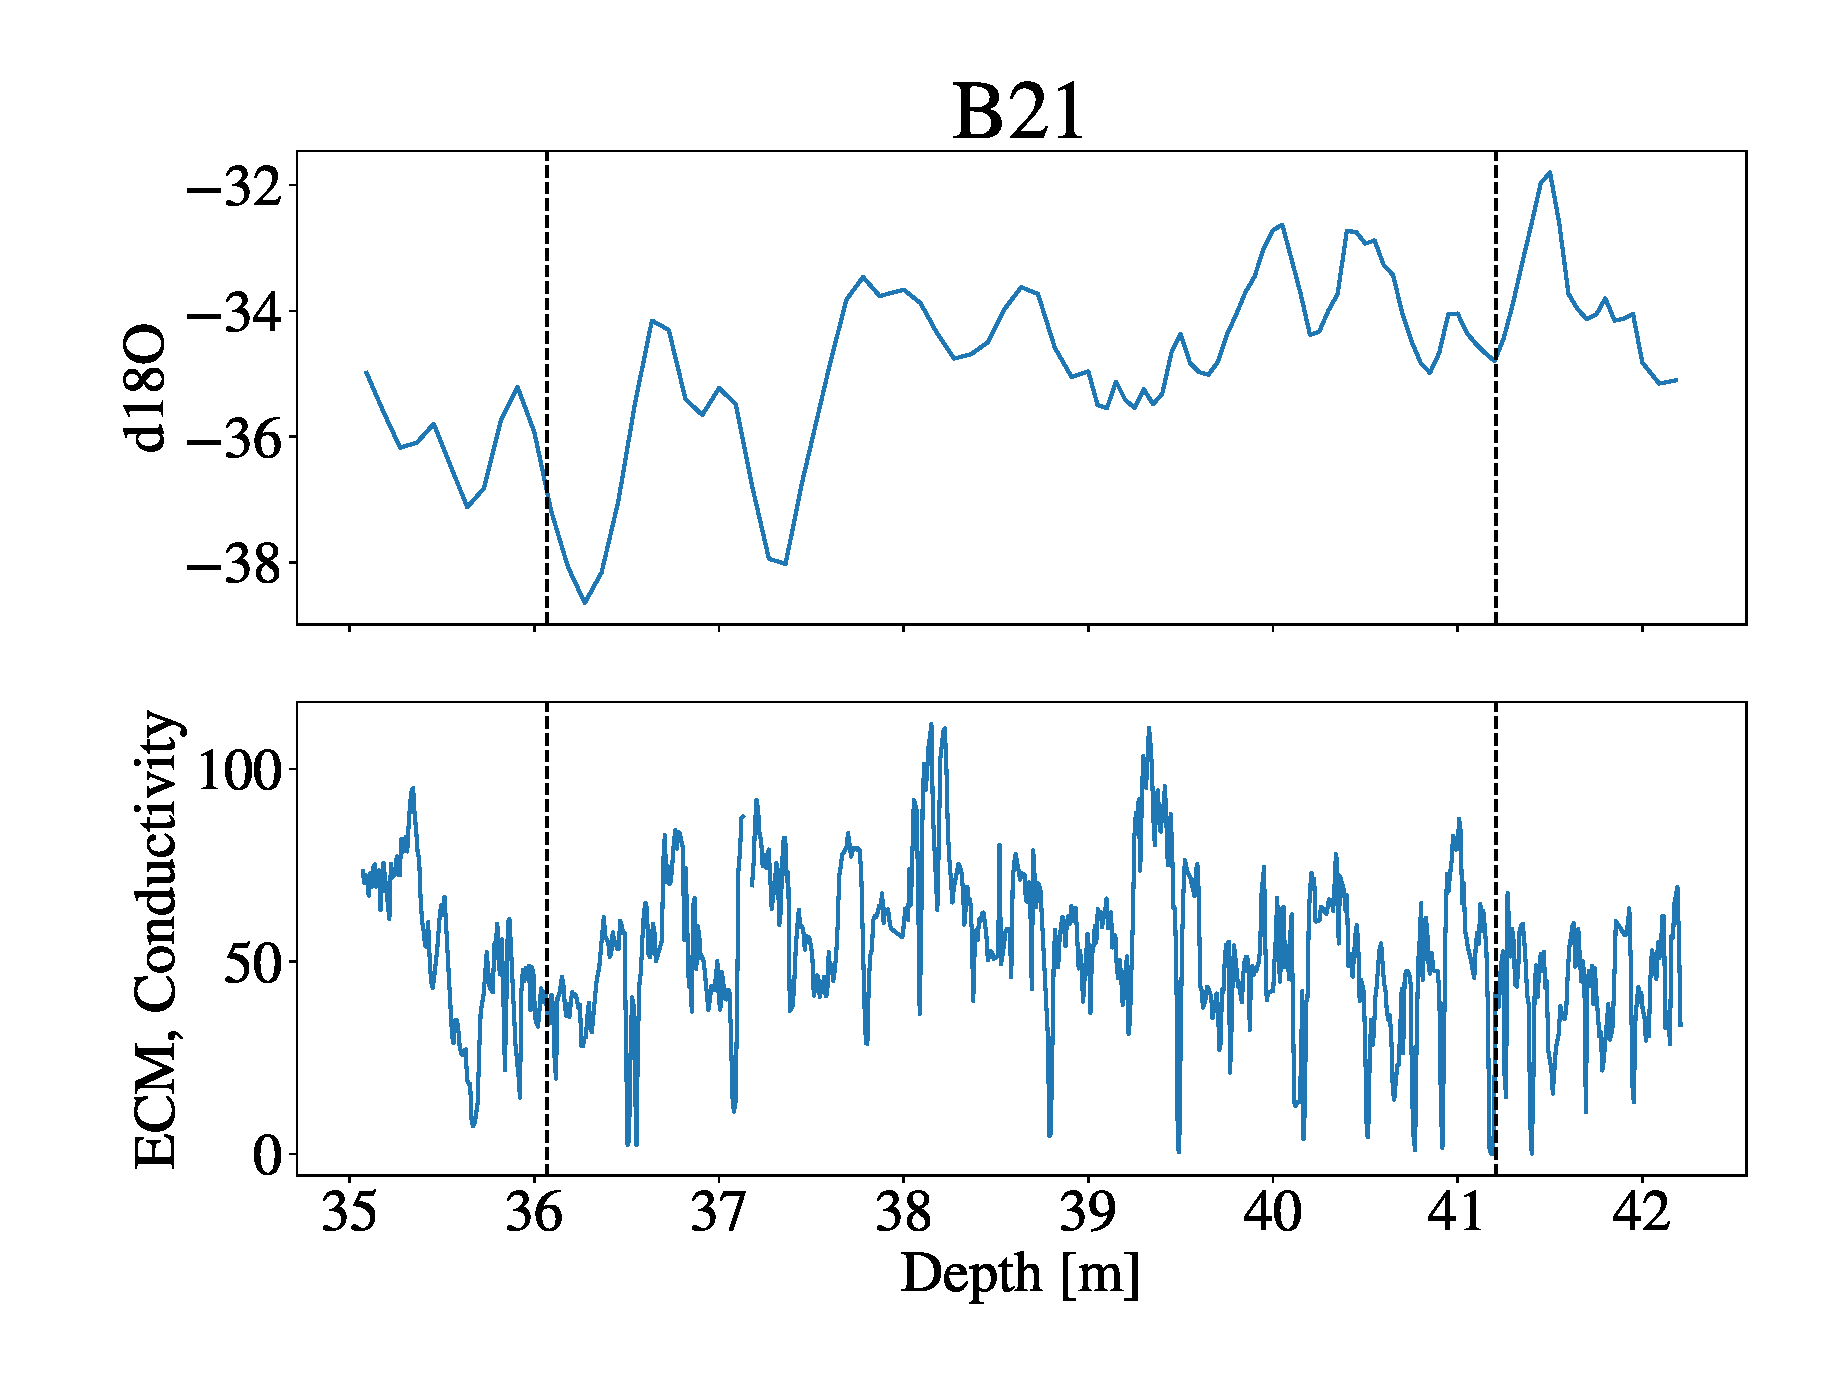
\includegraphics[width =0.3\linewidth]{Core_LT_B21.eps} & 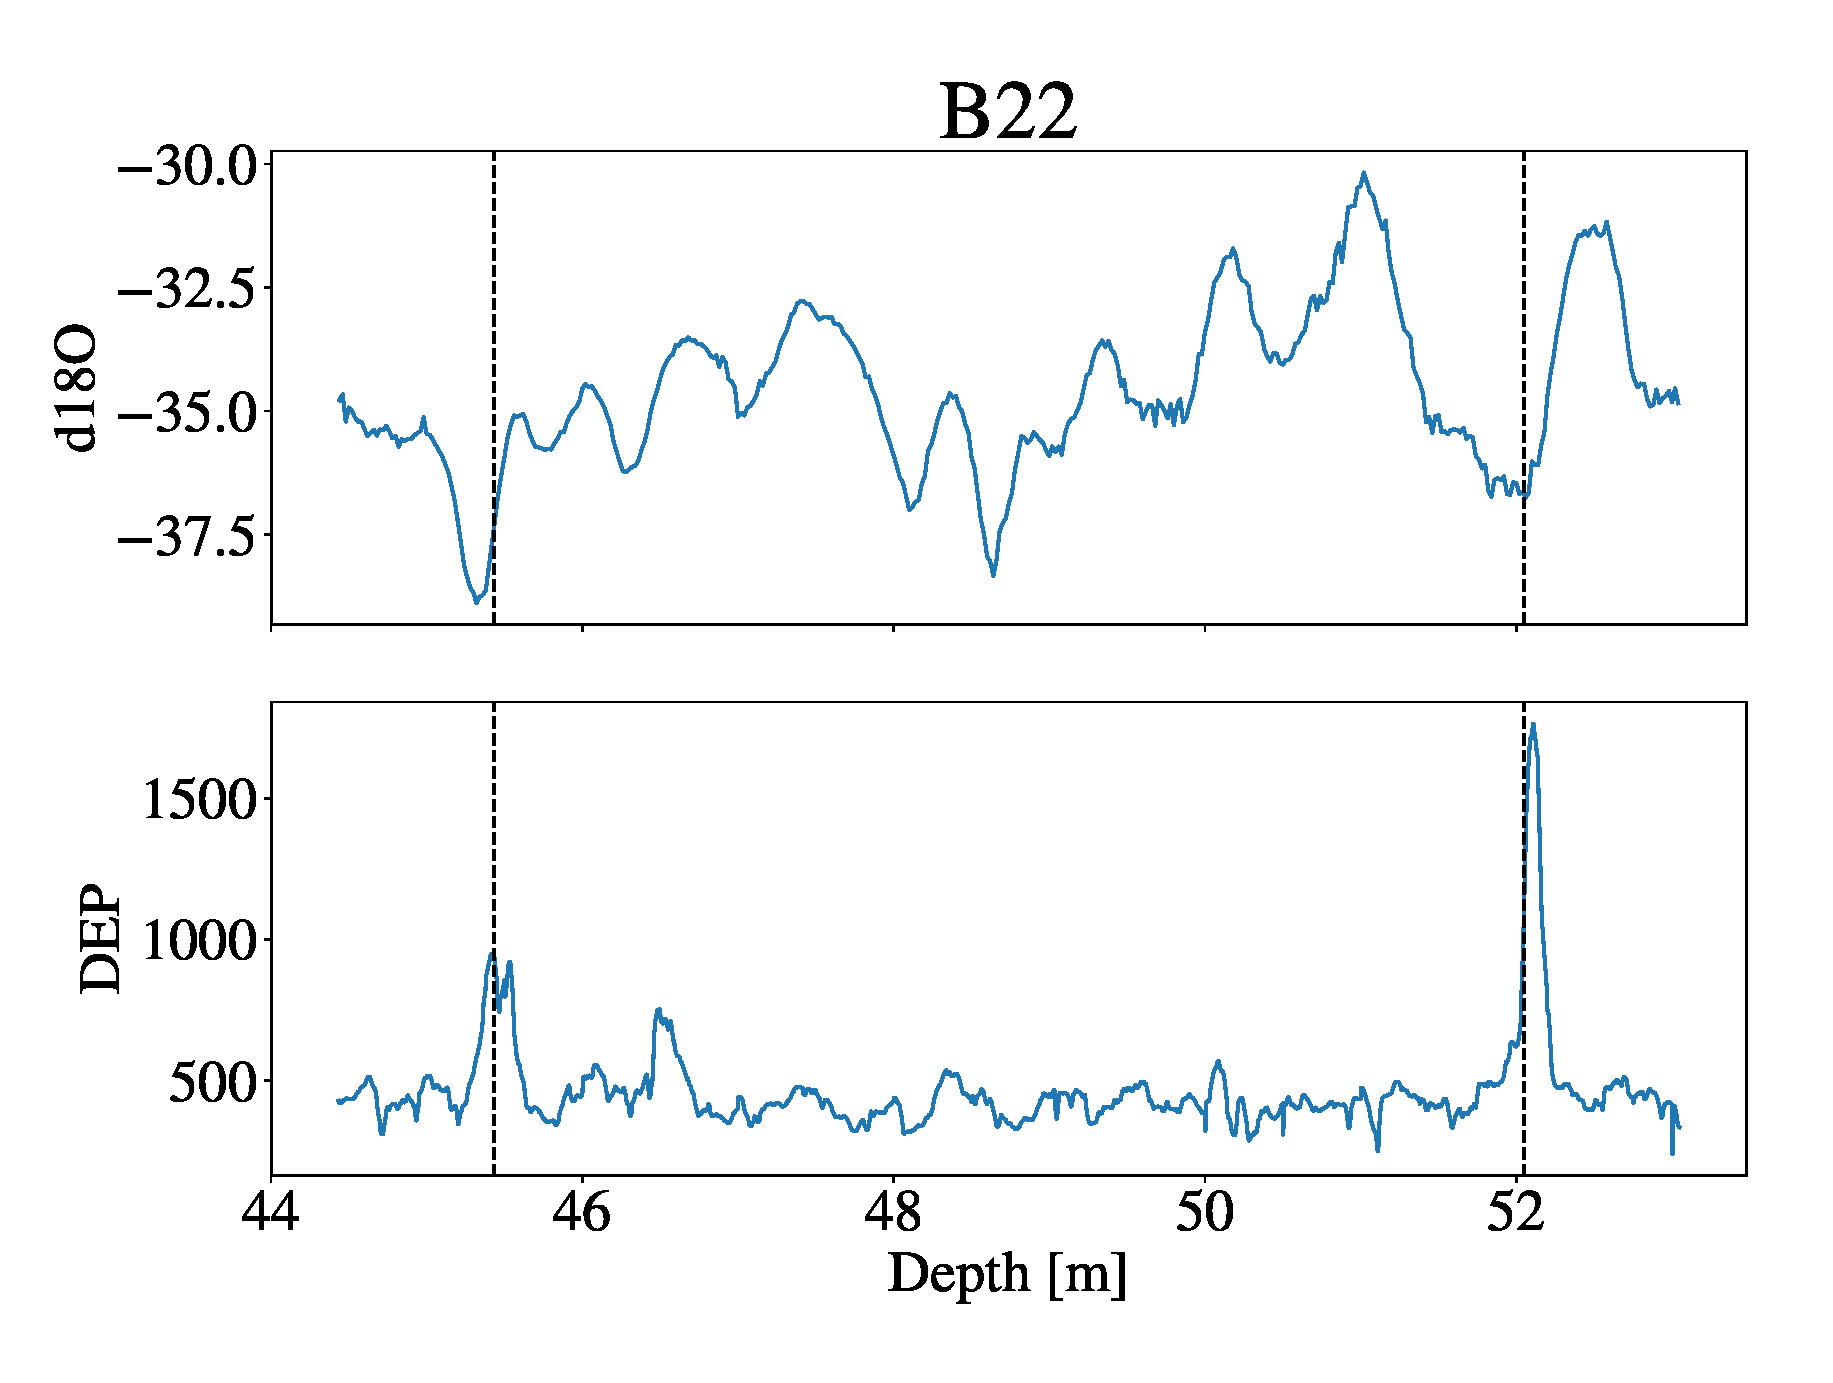
\includegraphics[width =0.3\linewidth]{Core_LT_B22.eps} \\	
				& & 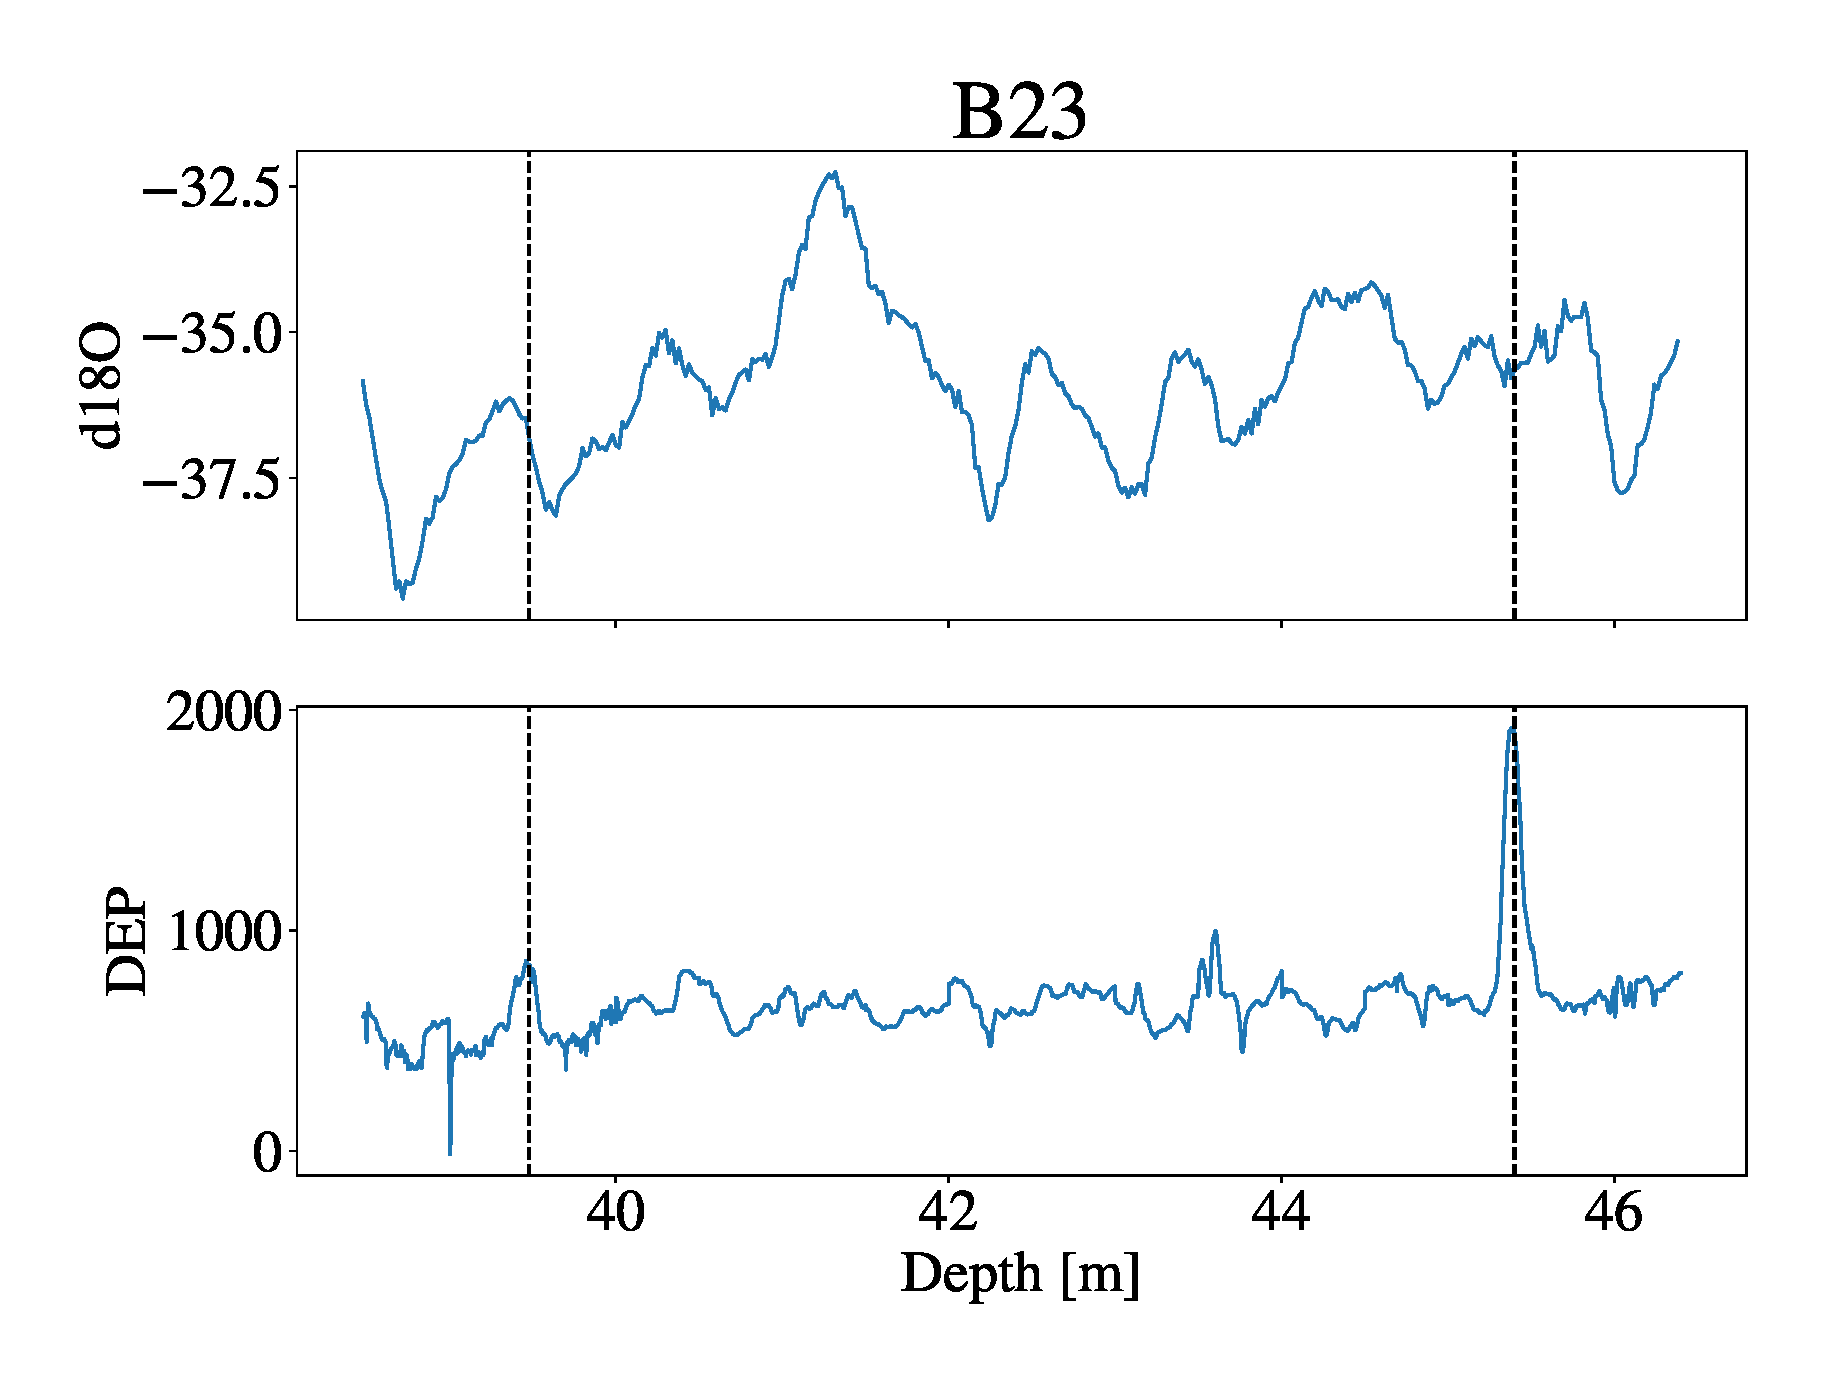
\includegraphics[width =0.3\linewidth]{Core_LT_B23.eps} \\
			\end{tabular}
		\end{table}
	\end{landscape}
\end{rotatepage}
\newpage
\begin{rotatepage}
	\begin{landscape}
		\begin{figure}[h]
			\centering
			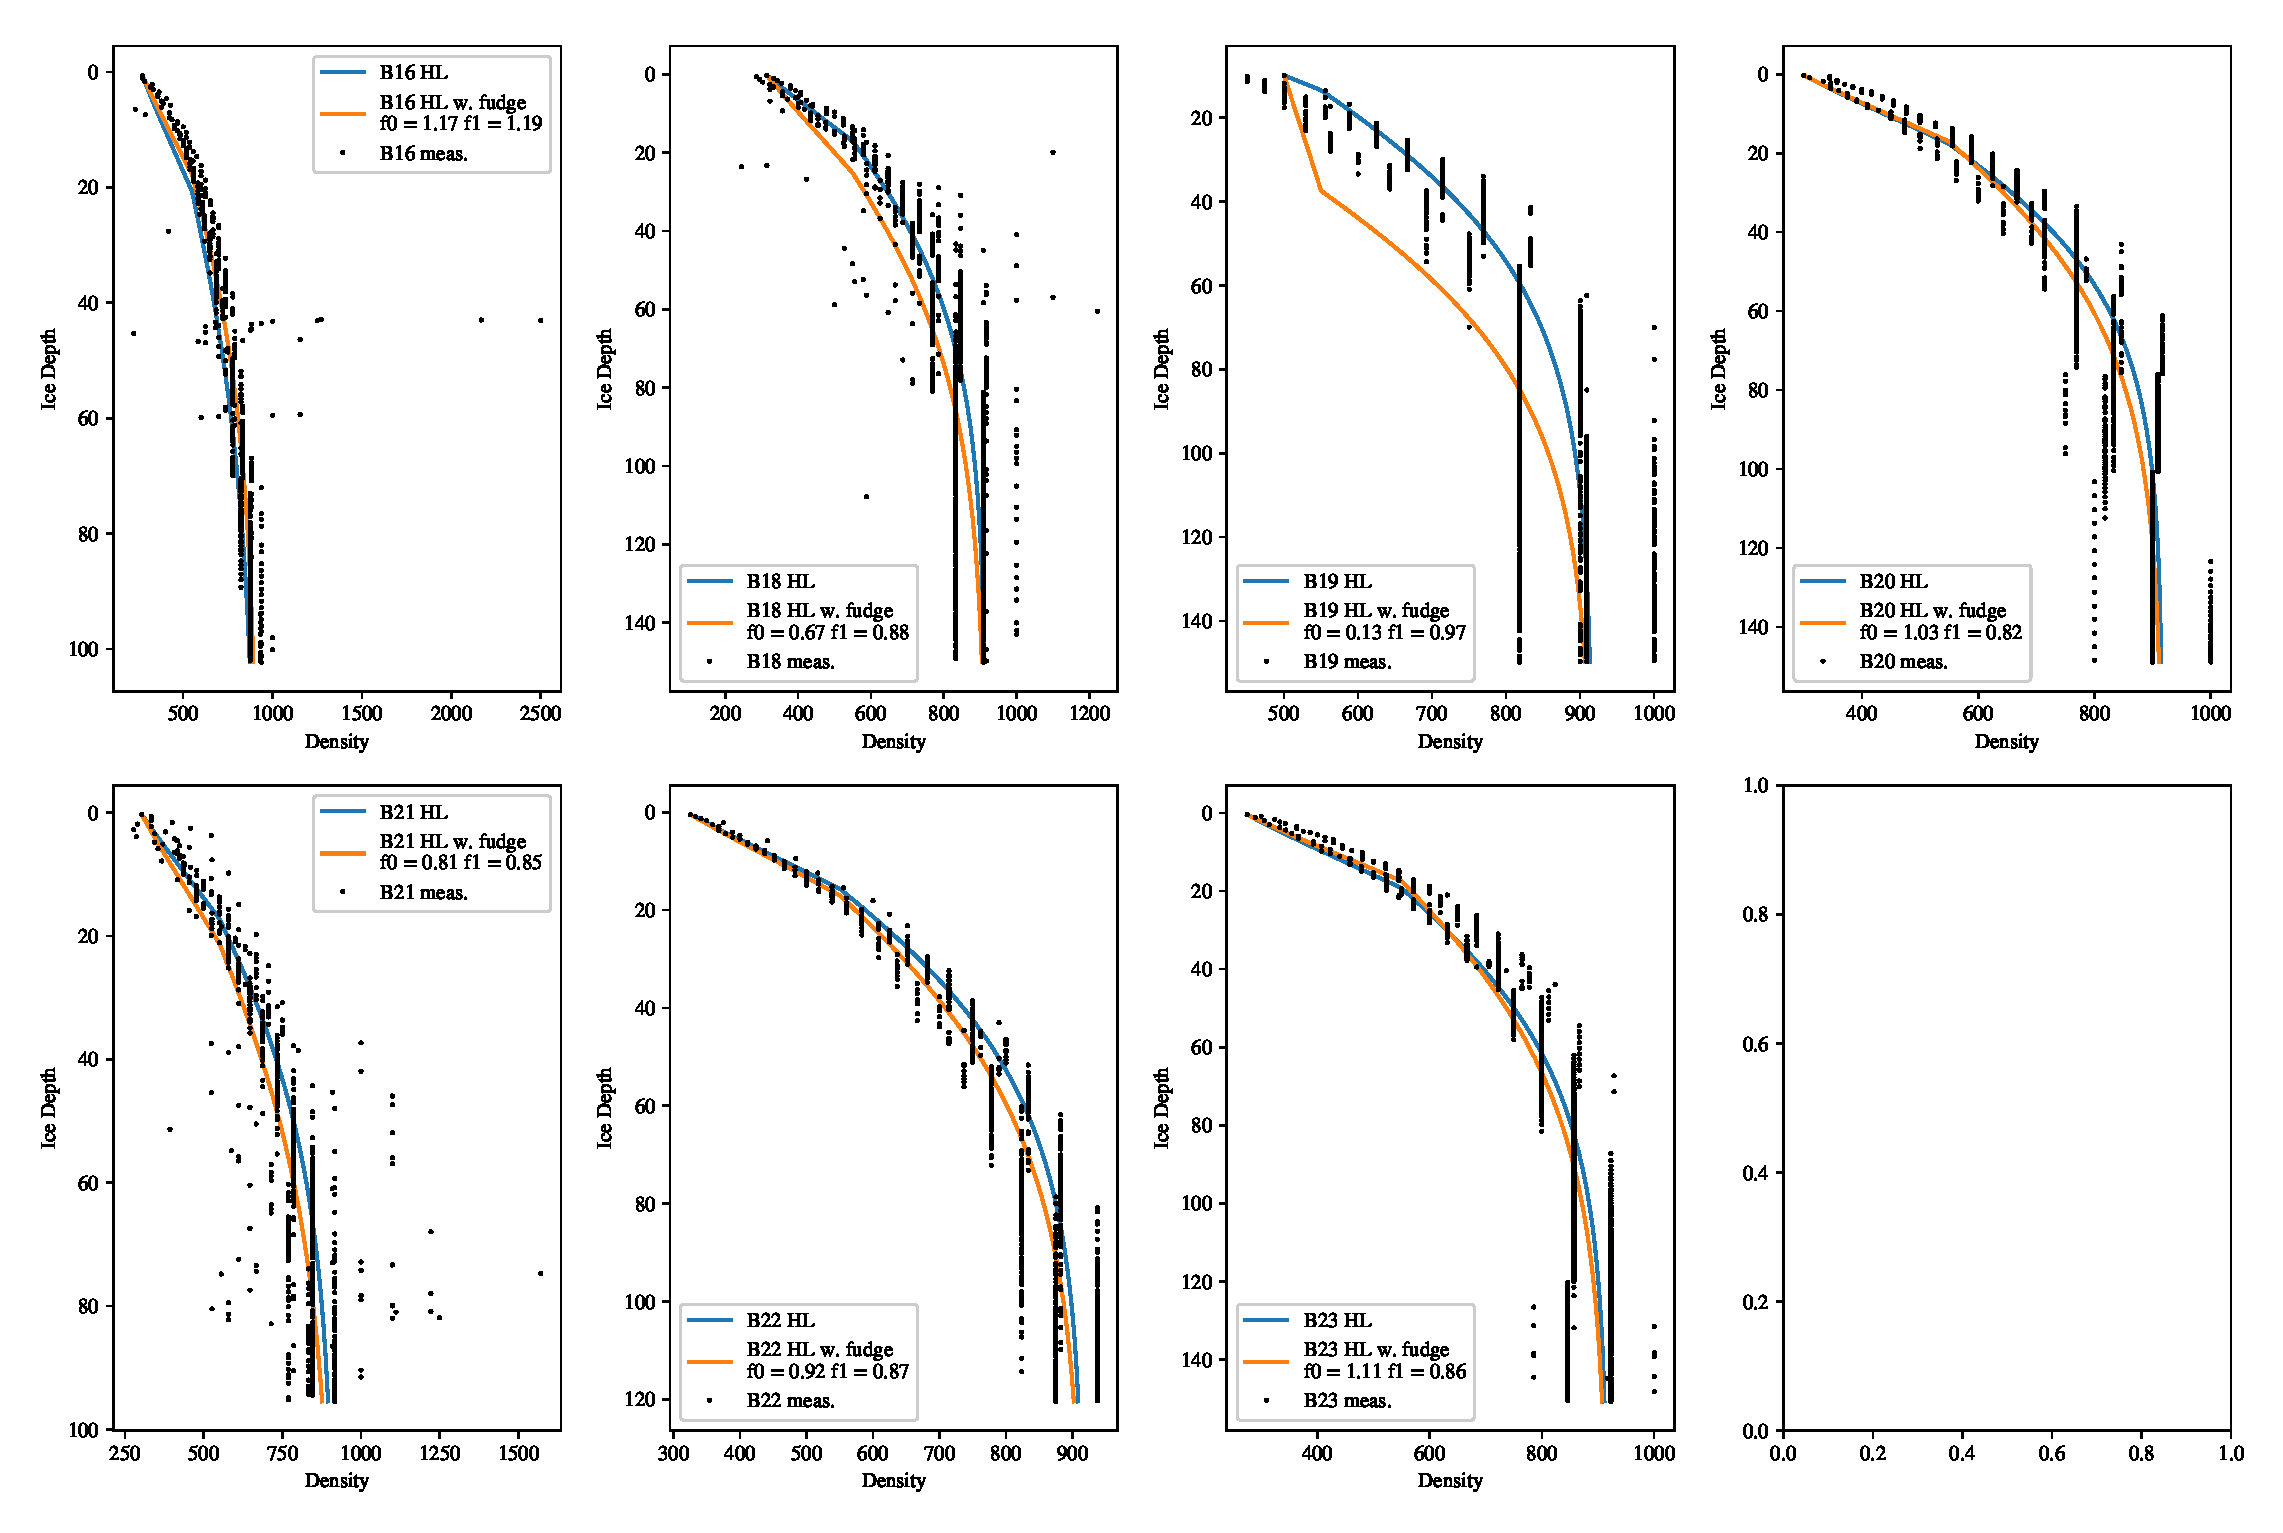
\includegraphics[width=1.5\textwidth]{fig_dens_B16B18B19B20B21B22B23.eps}
			\label{fig:dens}
			\caption{}
		\end{figure}
	\end{landscape}
\end{rotatepage}
\newpage
\begin{rotatepage}
	\begin{landscape}
		\begin{figure}[h]
			\centering
			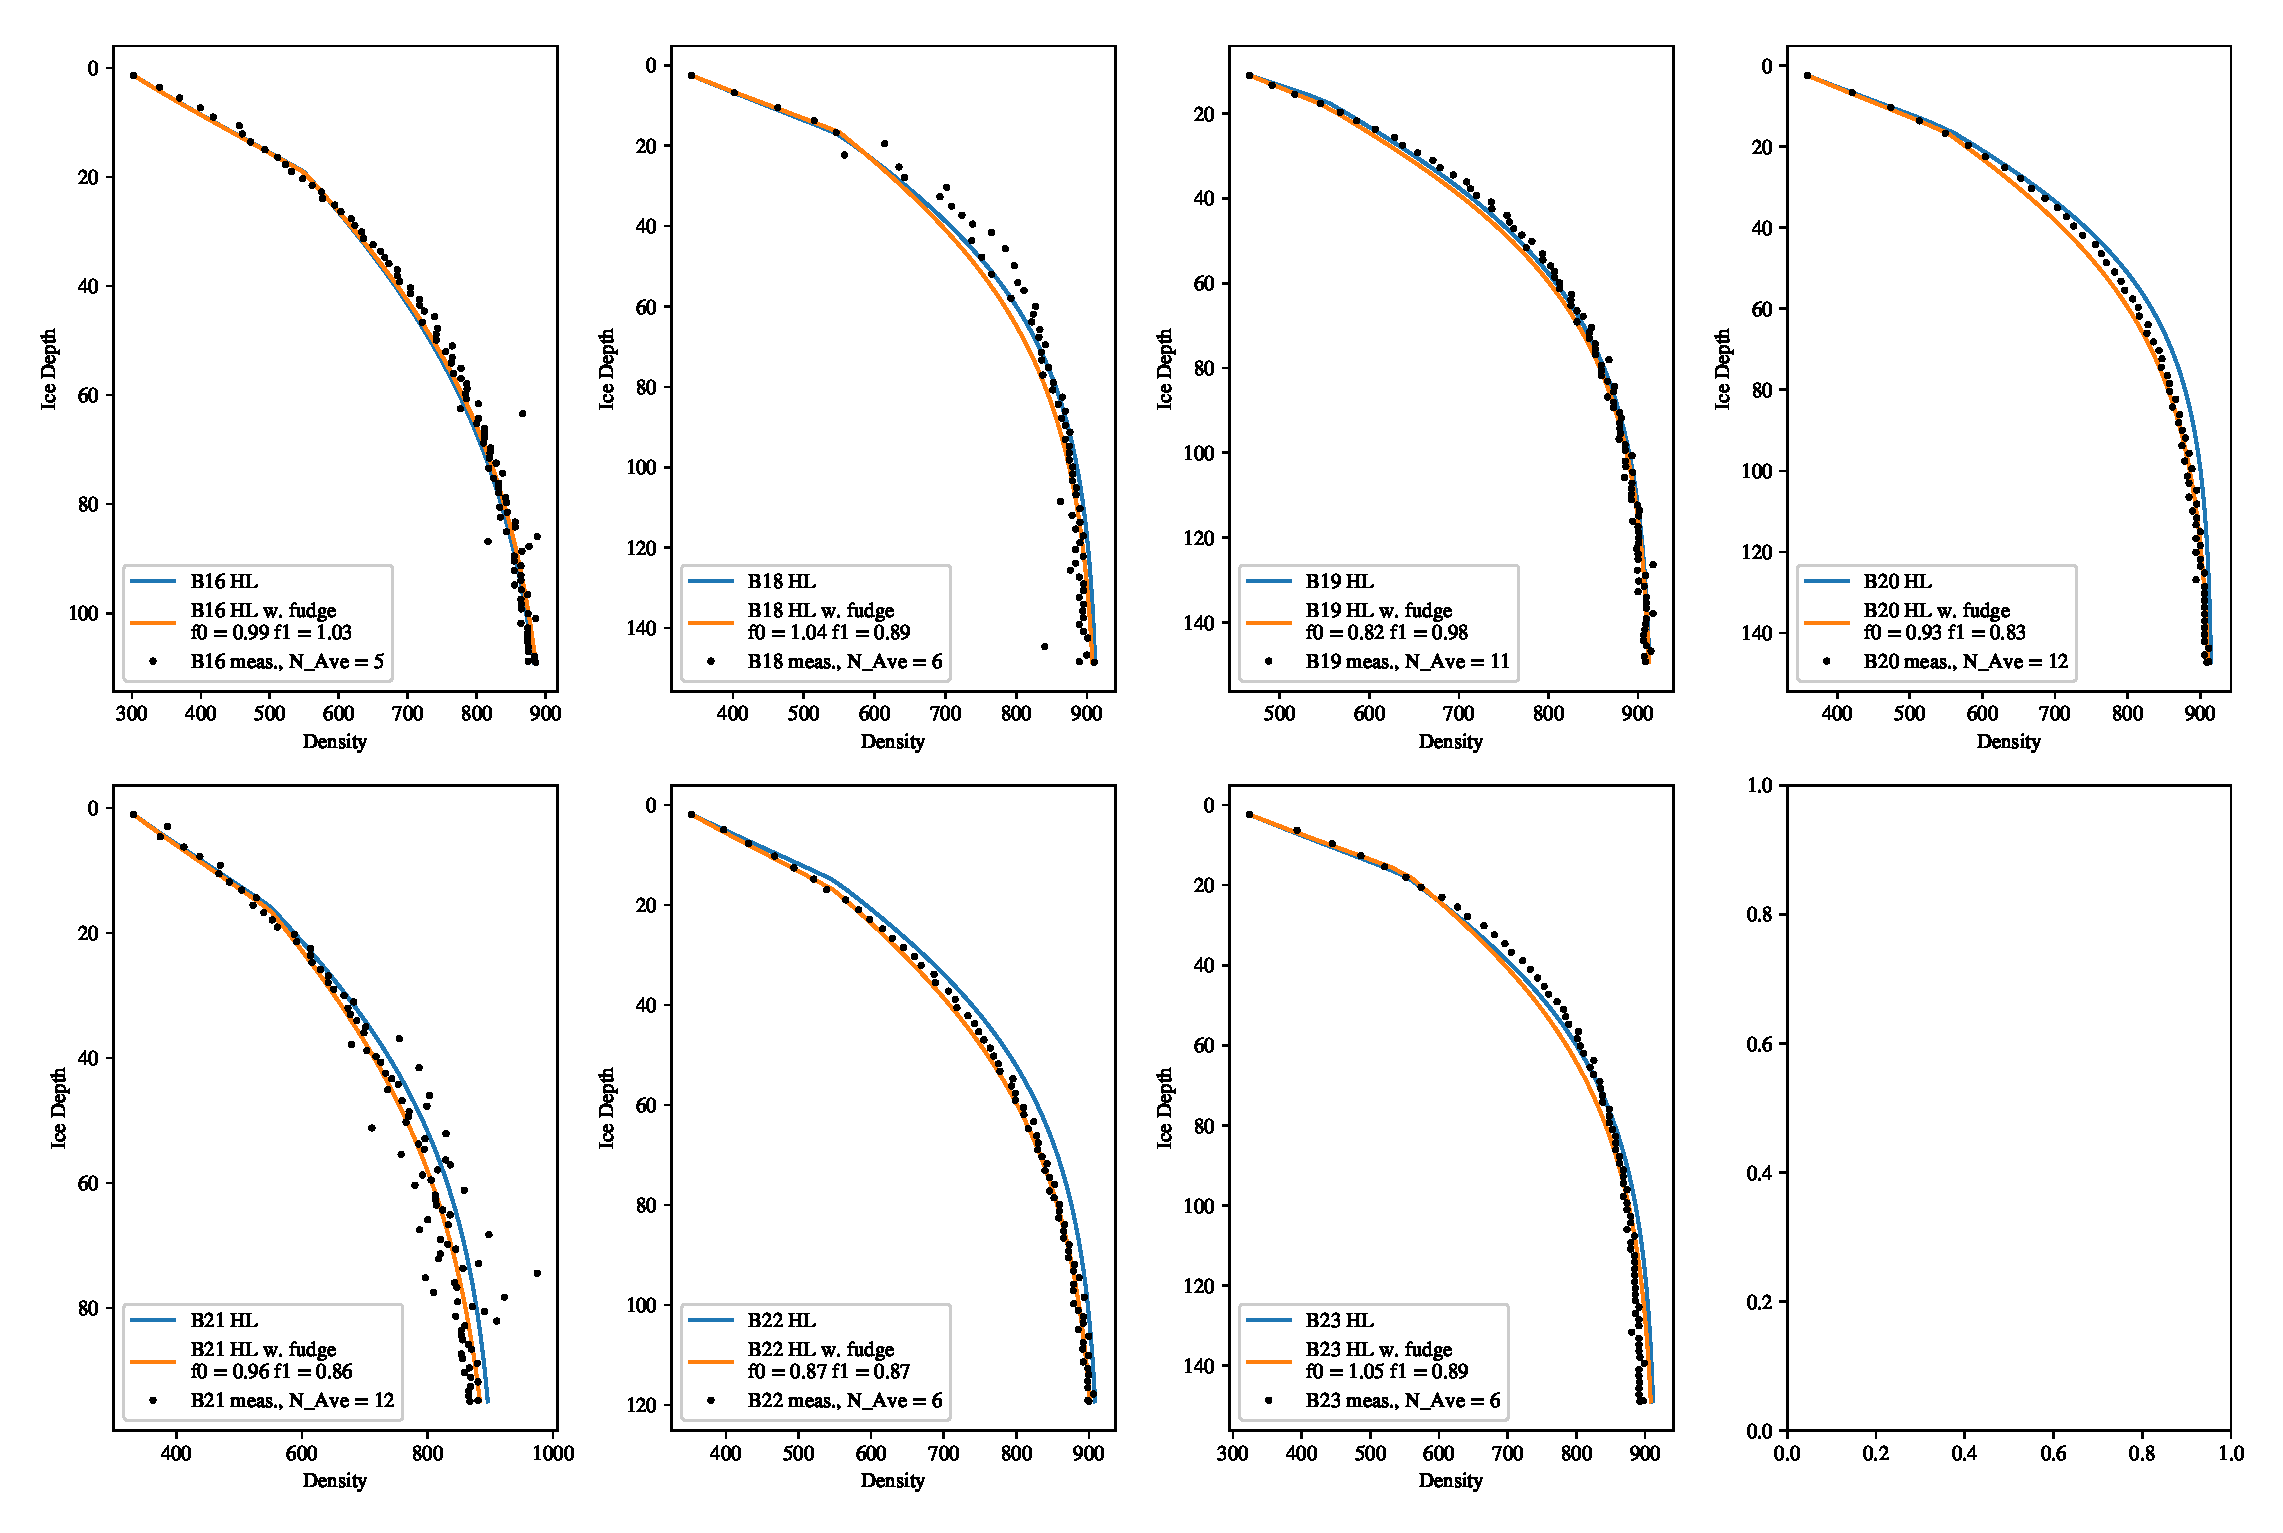
\includegraphics[width=1.5\textwidth]{fig_densAve_B16B18B19B20B21B22B23.eps}
			\label{fig:densAve}
			\caption{}
		\end{figure}
	\end{landscape}
\end{rotatepage}
\begin{figure}
	\centering
	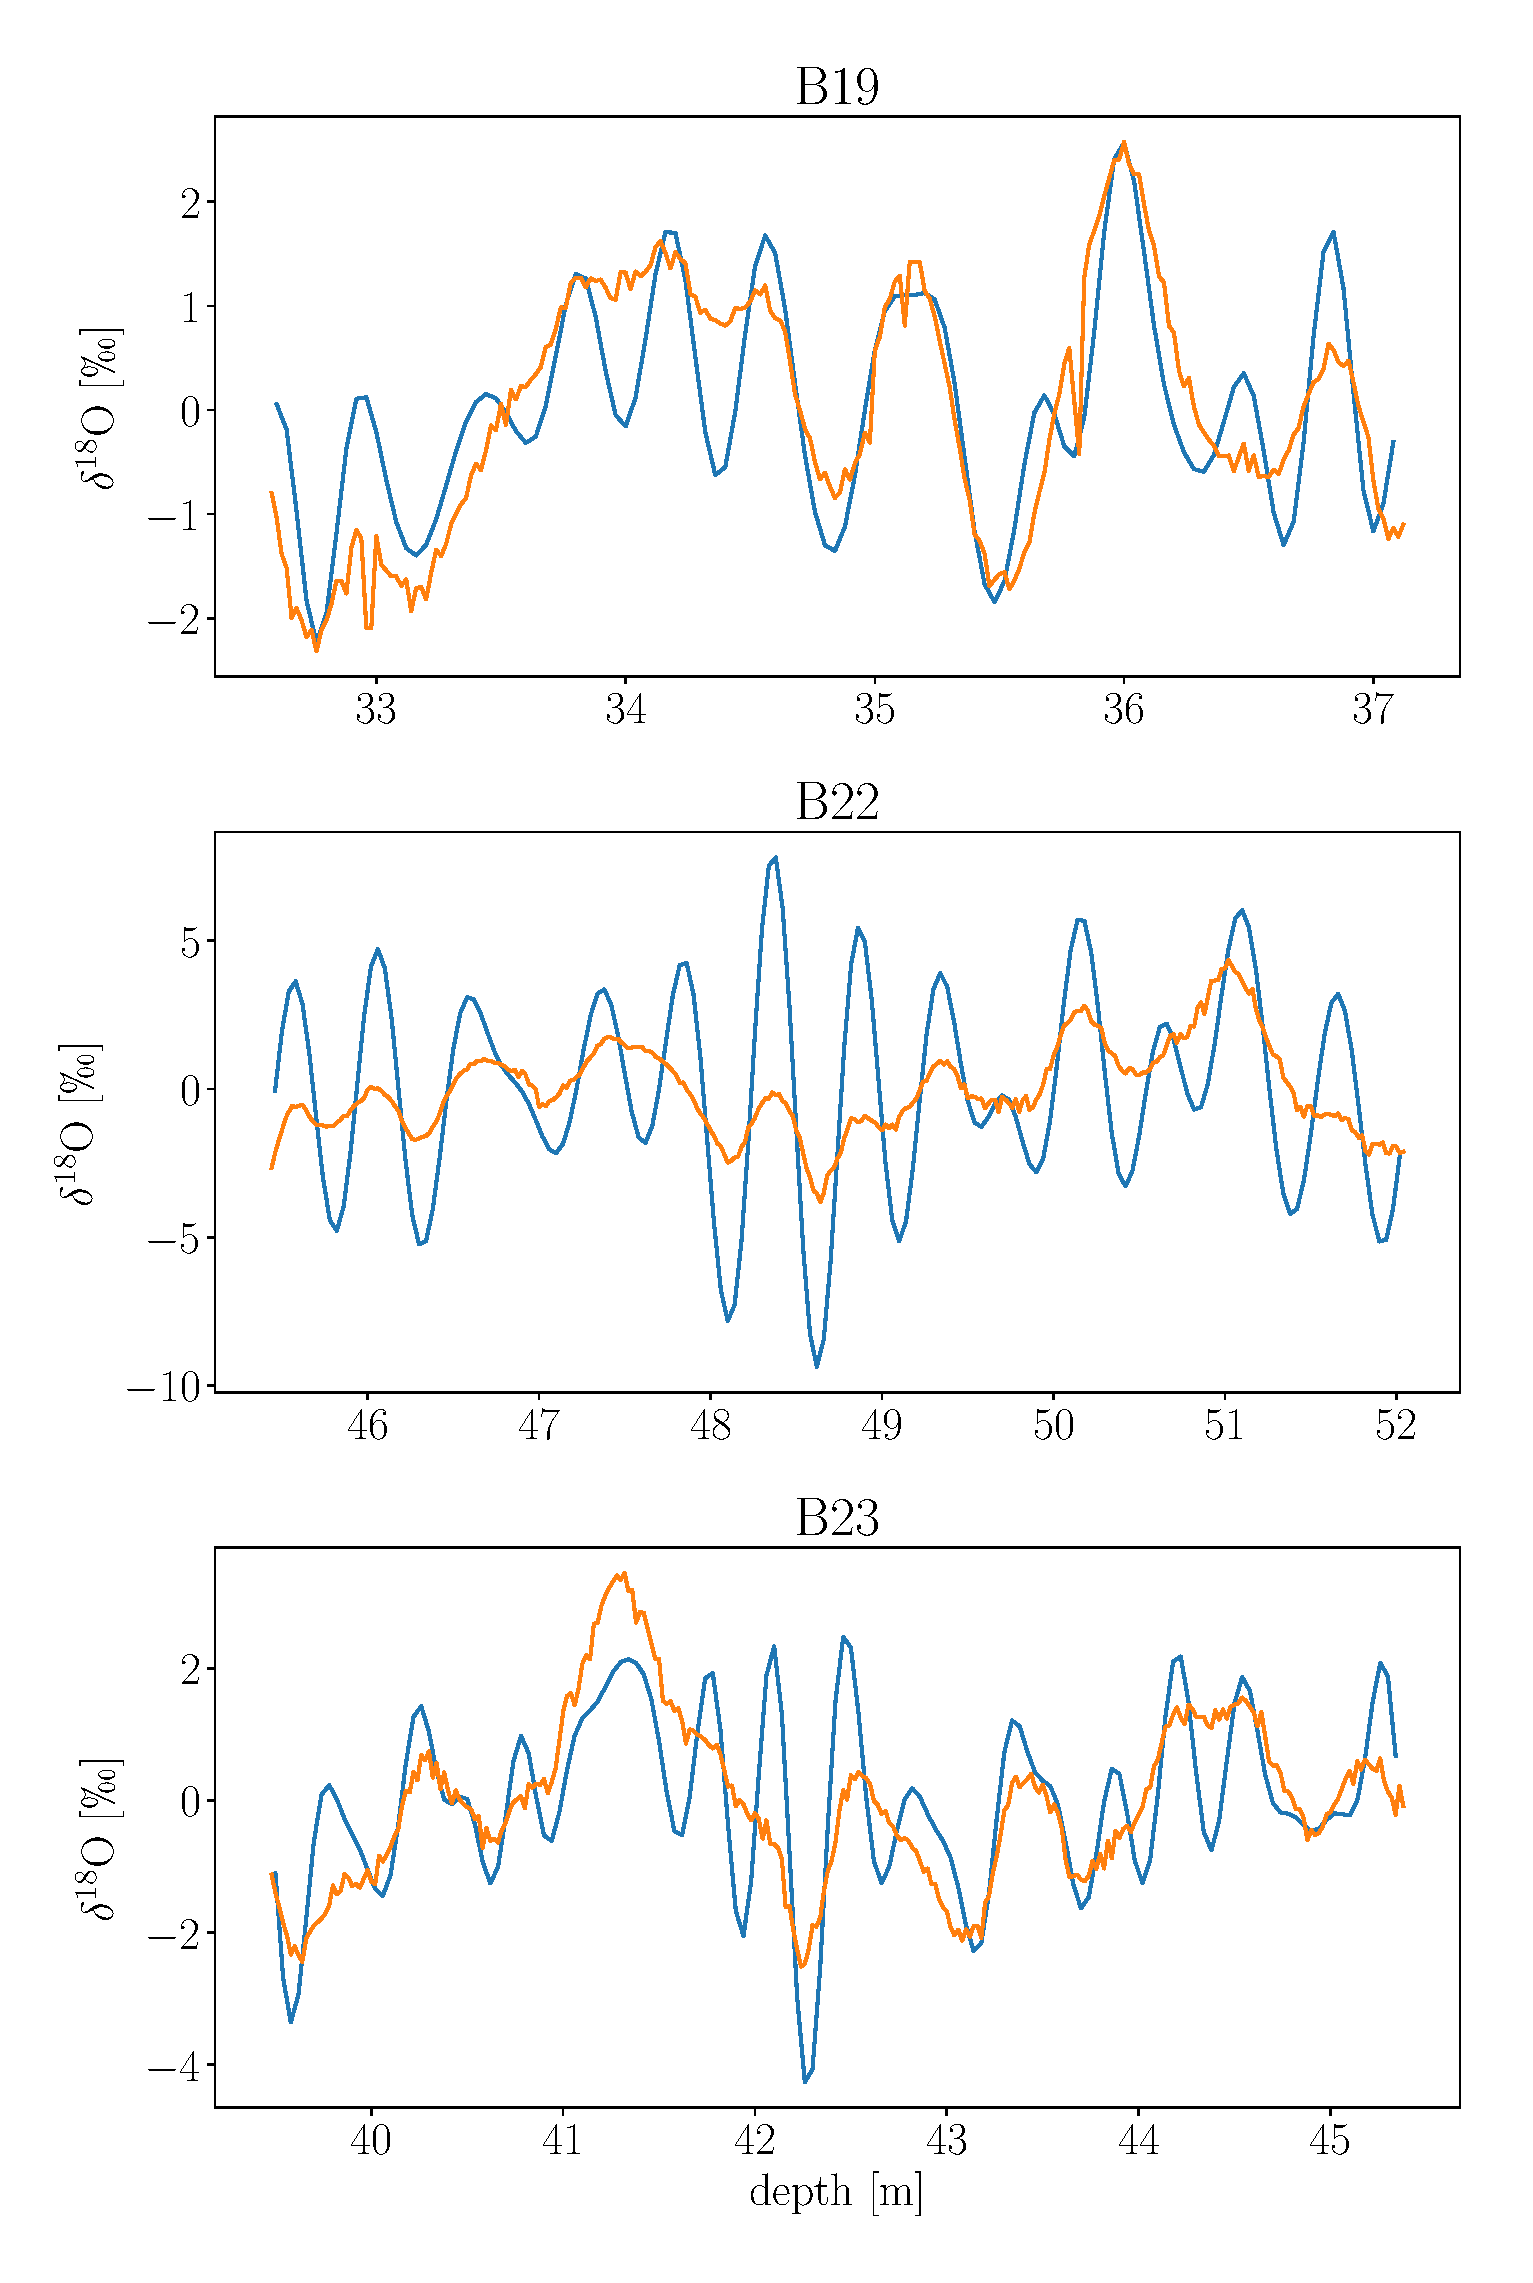
\includegraphics[width=0.8\textwidth]{deconvoluted__B19_B22_B23.eps}
	\label{fig:B19_B22_B23__decon}
	\caption{}
\end{figure}

\end{document}